\documentclass[12pt]{article}
\usepackage[
  a4paper,
  top=0.4cm,
  bottom=1.7cm,
  left=1.7cm,
  right=1.7cm,
  includehead,includefoot,
  heightrounded, % to avoid spurious underfull messages
]{geometry} 
\usepackage{wasysym} 
\usepackage{hyperref}
\usepackage{pdflscape}
{\renewcommand{\arraystretch}{2} %<- modify value to suit your needs

%delete the below to remove the numbering split by chapter
\usepackage{chngcntr}
\usepackage{caption}
\usepackage{subcaption}
%\counterwithin{figure}{section}
%\captionsetup[figure]{labelfont=bf,textfont=bf}

\usepackage{fancyhdr}
\fancyhf{} % clear all header and footers
\renewcommand{\headrulewidth}{0pt} % remove the header rule
\cfoot{\thepage}
\pagestyle{fancy}
\usepackage{wasysym} 
\usepackage{hyperref}
\usepackage{graphicx}
\usepackage{placeins}
\usepackage{epsfig}
\usepackage{epstopdf}
\usepackage{color}

%change the font
\renewcommand{\familydefault}{\sfdefault}

%creates the marker command
\newcommand{\marker}[1]{\color{red}\textbf{#1}\color{black}}

%% Handles the info and warning boxes
\usepackage{mdframed}
\newmdenv[
	linewidth=2pt,
	leftmargin=0.3cm,
	rightmargin=0.3cm,
	leftline=false,
	rightline=false,
	linecolor=red,
	frametitle={\lightning\ Warning!},
	frametitlefont=\color{red}\bfseries
]{warningBox}
\newmdenv[
	linewidth=2pt,
	leftmargin=0.3cm,
	rightmargin=0.3cm,
	leftline=false,
	rightline=false,
	linecolor=blue,
	frametitle={\checked\ Note},
	frametitlefont=\color{blue}\bfseries
]{infoBox}

\newcommand{\myref}[1]{\ref{#1} {\scriptsize(Page \pageref{#1})}} 

\title{\vspace{-1cm}\textbf{Dover War Memorial Project - User Guide}\vspace{-1cm}}
\date{}
\author{}
%%%%% document start
\begin{document}

\maketitle

This document acts as a user guide for someone who will be also performing administration functions (i.e. it's not for the general public). It will identify features of each page, and how to perform all the actions required to maintain and update the website.

\tableofcontents

\section{Notes}
Buttons on screen are labelled in \textit{italics}, with text to be entered or displayed in \texttt{monospace}. Any \textit{Edit}, \textit{Add} or \textit{Delete} buttons in screenshots are not displayed if the user is not logged in. Numbers in red, for example \marker{1}, point to a reference of the relevant figure.

\begin{infoBox}
Some information may be of interest and is displayed in this type of box.
\end{infoBox}

\begin{warningBox}
More serious information may be displayed in a box similar to this.
\end{warningBox}

\newpage

\section{Navigation \& Login}
There are two main menu bars on the site. These are displayed on every single page, with the top bar gaining an extra row when logged in. The text disappears when viewed on mobile, for space reasons. The home page contains the same content as before, along with some dynamic data: a summary of the most recent news article and the names of any casualties that died on this day.

\subsection{What does the Home Page do?}
Figure~\myref{fig:home} shows the home page as viewed when not logged in. \marker{1}\ links back to the home page, \marker{2}\ navigates to the Latest News area (Section~\myref{sec:siteUpdate}), \marker{3}\ to the Casualty Index (Section~\myref{sec:casualtyIndex}), \marker{4}\ to the Articles area (Section~\myref{sec:articles}), \marker{5}\ the Search area (Section~\myref{sec:search}) and \marker{6}\ to the Contact Us page. At the bottom of the page, these links are reproduced, with the addition of \marker{7}, which navigates to the Login page (Section~\myref{ssec:login}). Other areas on the page are the latest news article (\marker{8}), the list of casualties who died today (\marker{9}) and the main narrative (\marker{10}).

\begin{figure}[h]
  \centering
 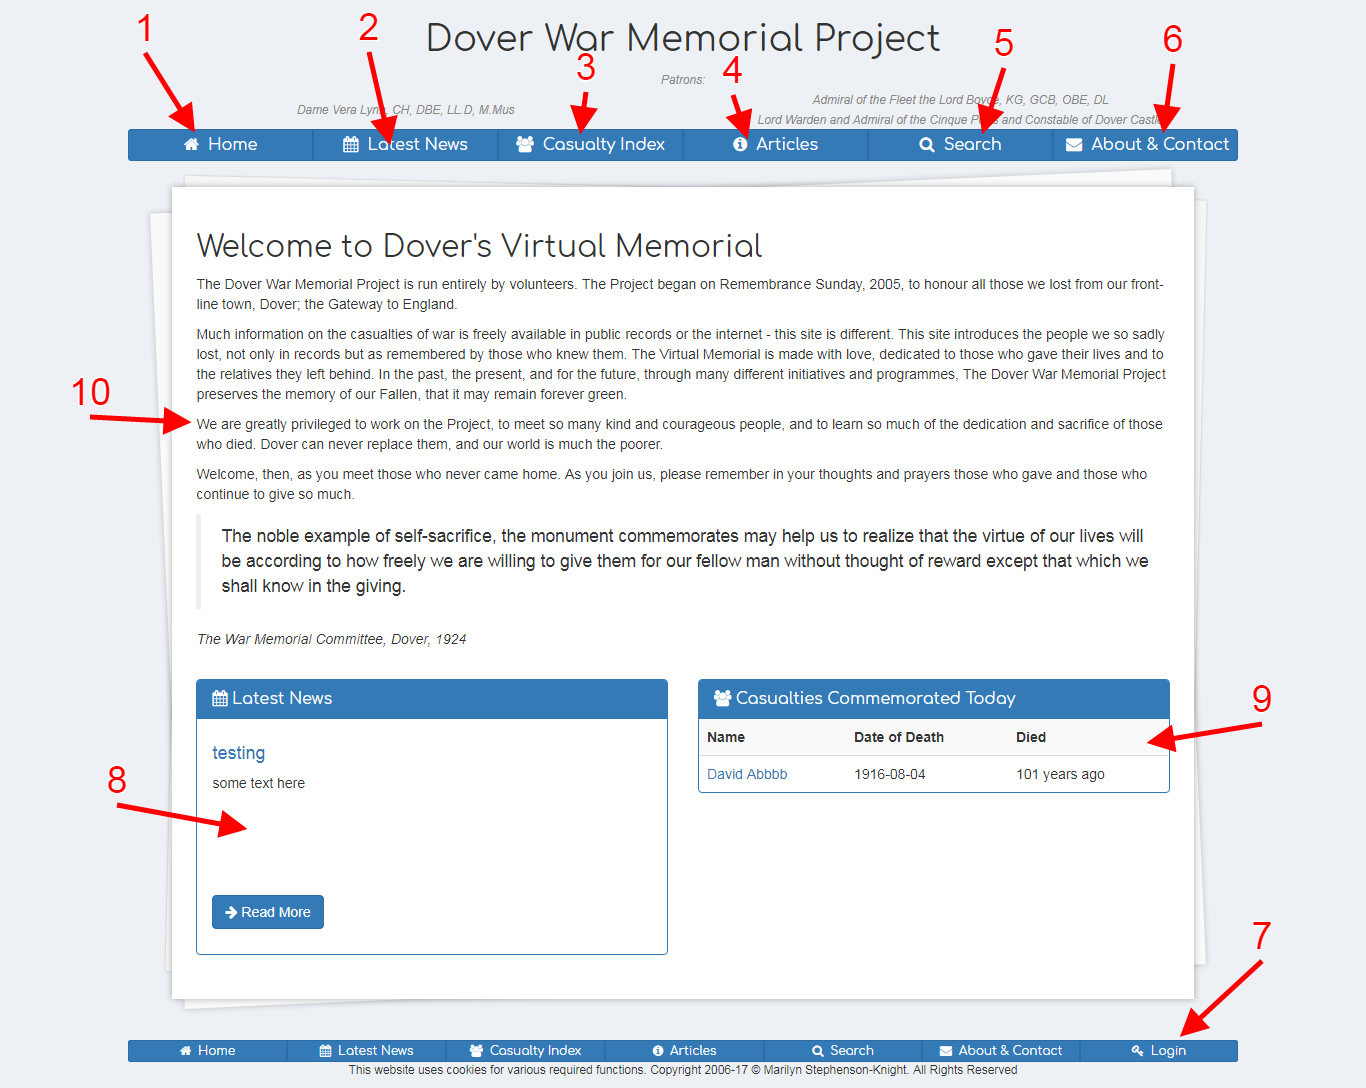
\includegraphics[width=.9\textwidth]{pics/home.png}
	\caption{Home Page}\label{fig:home}
\end{figure}

\newpage
\FloatBarrier
\subsection{How do I login?}\label{ssec:login}
To login, click the \textit{Login} button on the bottom menu bar (see \marker{7}\ on Figure~\myref{fig:home}). The login page is then loaded (Figure~\myref{fig:login}), which allows the user to login to the site to make various changes. \marker{1}\ is where the username must be entered with \marker{2}\ being the password field. \marker{3}\ submits this information.

\begin{warningBox}
There is no way of resetting your username or password, so ensure that you remember it
\end{warningBox}

\begin{figure}[h]
  \centering
 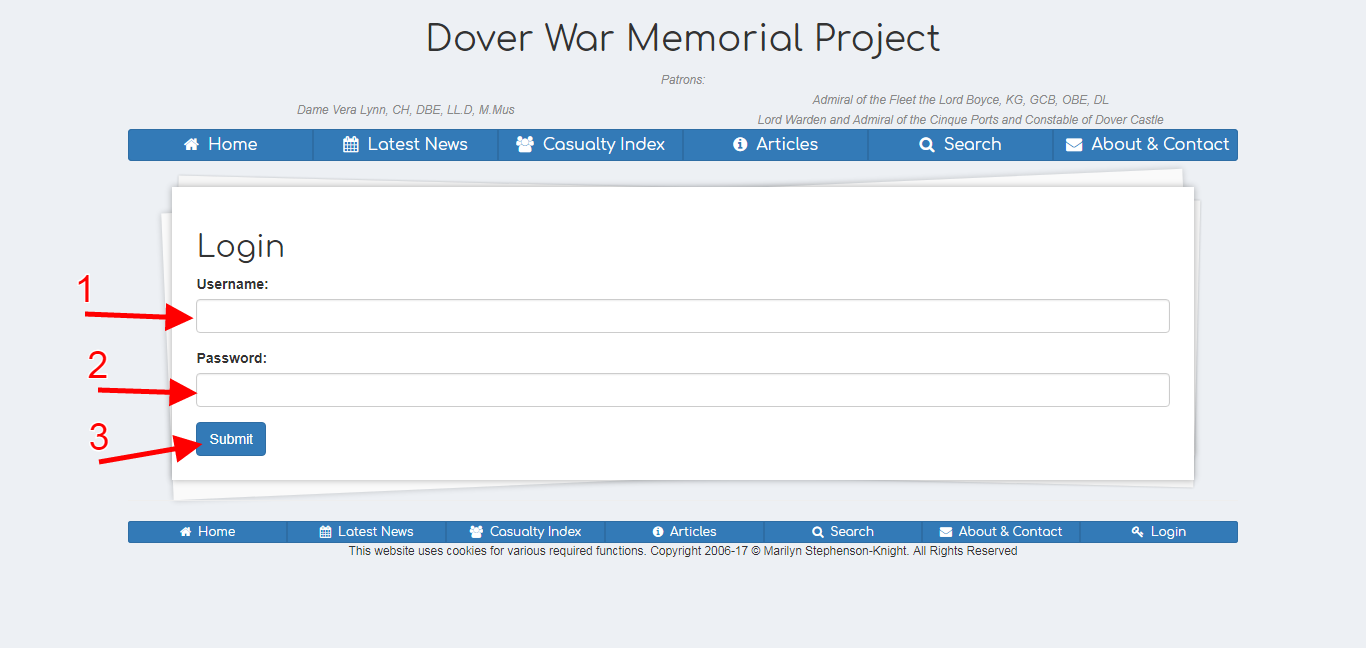
\includegraphics[width=.9\textwidth]{pics/login.png}
	\caption{Login Page}\label{fig:login}
\end{figure}

\newpage
\FloatBarrier
\subsection{How does the Home Page look after Login?}
Once a user has logged in, menu bars change. The top menu bar gains another row, with the login button on the bottom bar being replaced with a logout button, as can be seen in Figure~\myref{fig:home_login}. \marker{1}\ shows the currently logged in user, \marker{2}\ navigates to the config page (Section~\myref{sec:config}) and \marker{3}\ the admin help page (where this document is stored). \marker{4}\ and \marker{5}\ allow the user to logout. \marker{6} allows the user to edit the narrative text. These appear in numerous places across the site.

\begin{figure}[h]
  \centering
 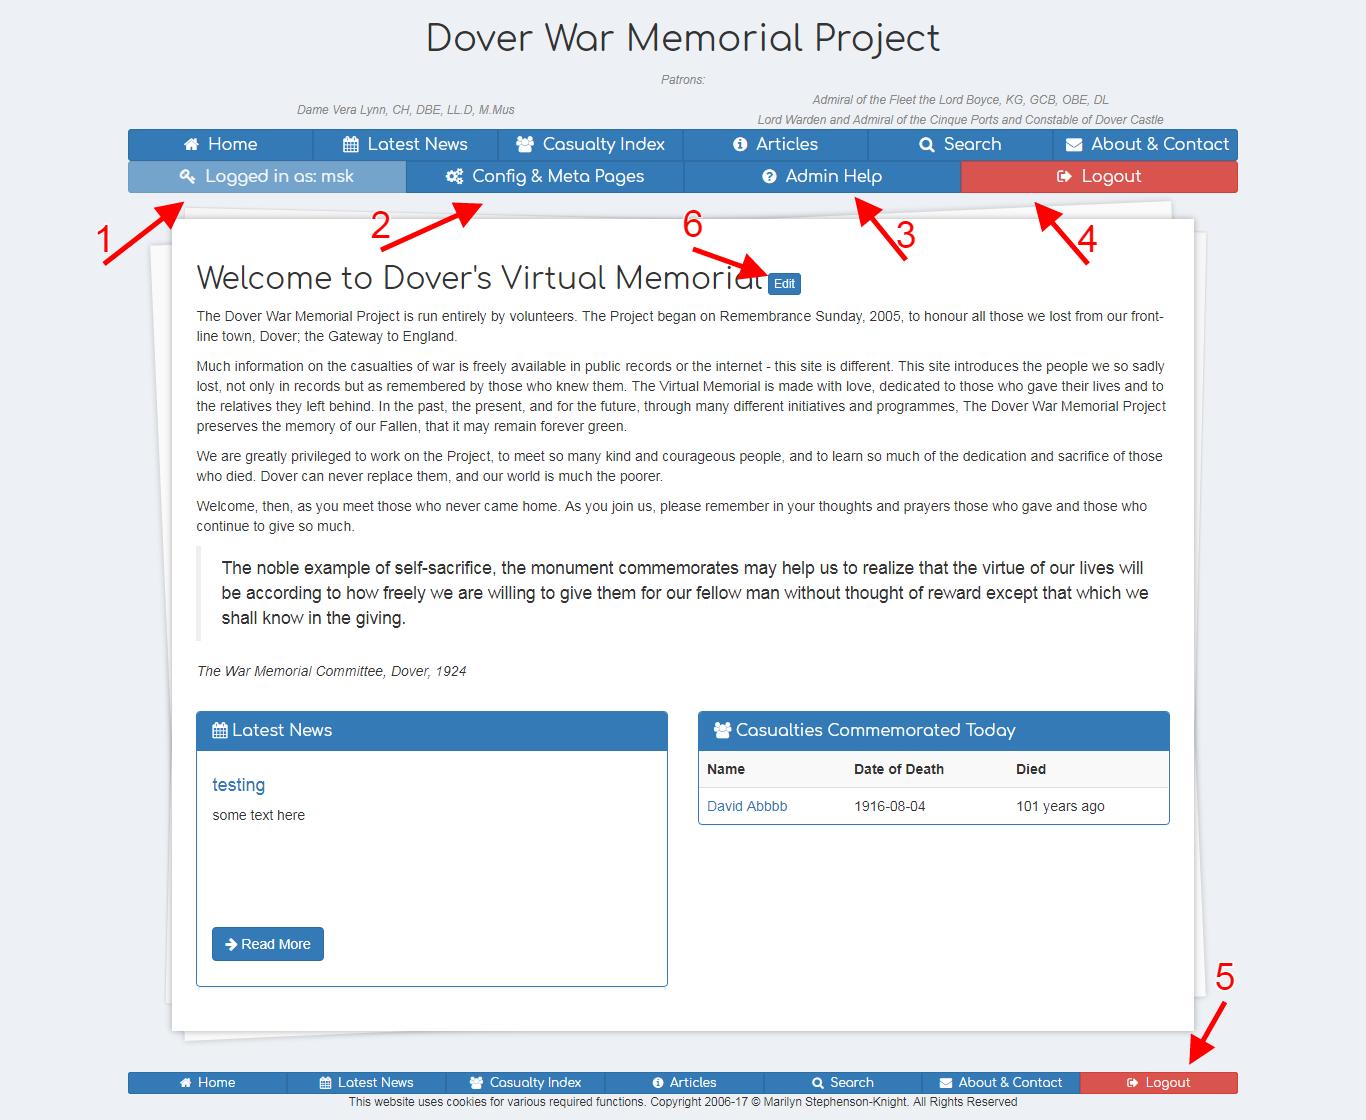
\includegraphics[width=.9\textwidth]{pics/home_login.png}
	\caption{Home Page after Login}\label{fig:home_login}
\end{figure}

\newpage
\FloatBarrier
\section{Site Updates}\label{sec:siteUpdate}
This section of the site contains two areas: Latest News, and a Change Log. The latest news section is for interesting updates and events that you may wish to bring attention to, in a similar way to the current latest news page. The most recent news article is also displayed on the home page.

The Change Log is a list of all the changes on the site (or rather, all the changes when you have entered a description of the change). This allows those visitors who wish to know what exactly is changing and when the ability to do so. It's also quite useful to show that the site is ``fresh'' and being regularly updates.

\subsection{How do I view a List of Updates?}\label{ssec:view_updates}

Navigate to Site Update section, by clicking the \textit{Latest News} link in either menu bar. A list of this year's updates will show, in a similar fashion to Figure~\myref{fig:view_updates}.

\begin{figure}[h]
  \centering
 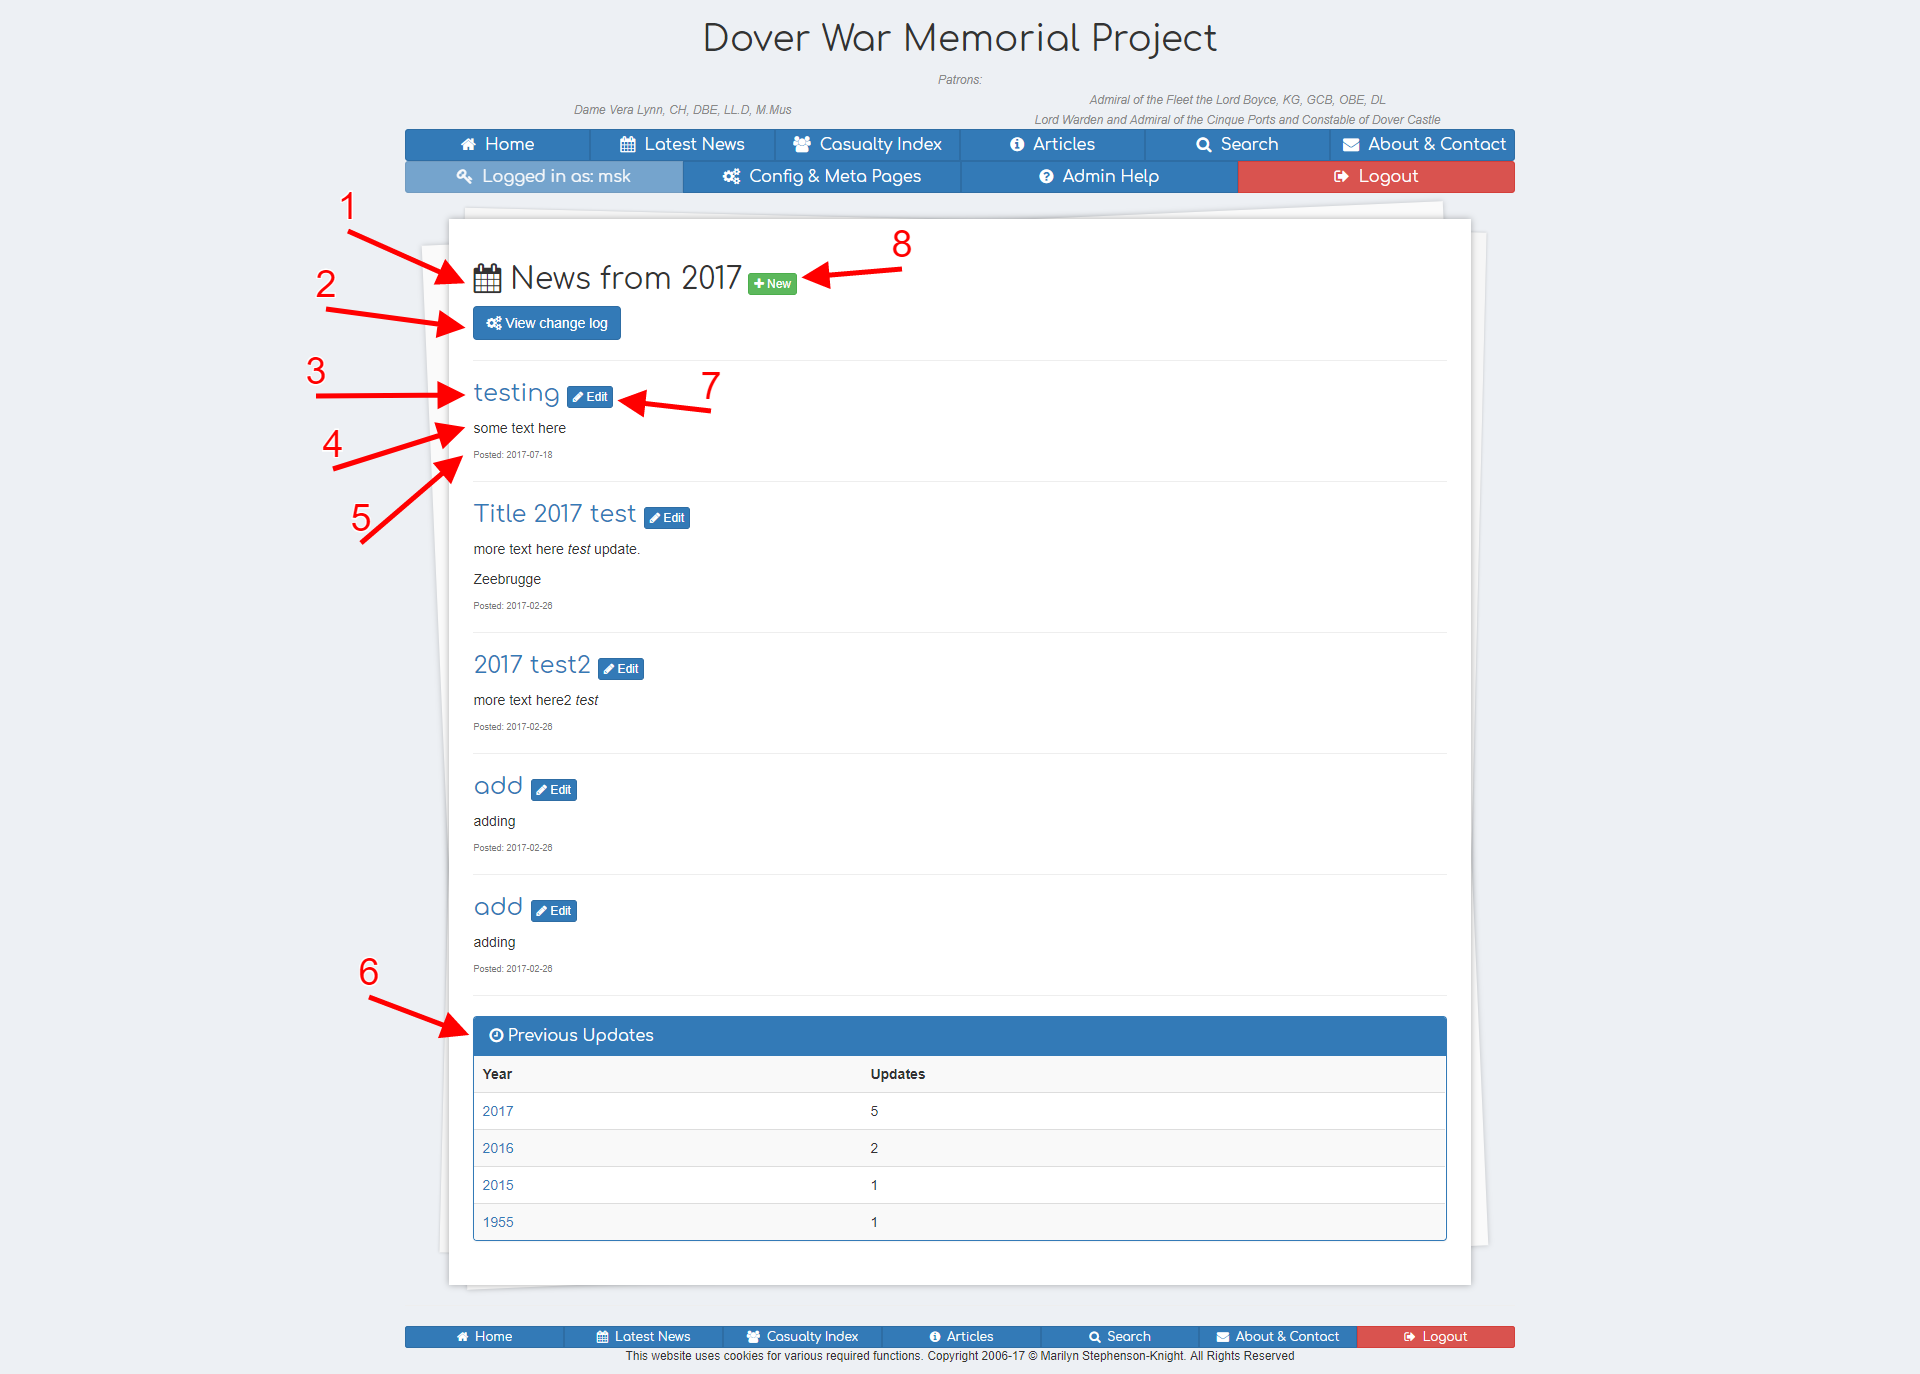
\includegraphics[width=.9\textwidth]{pics/view_updates.png}
	\caption{List of Site Updates}\label{fig:view_updates}
\end{figure}

\marker{1}\ indicates which year's updates are being shown, with \marker{2}\ providing a link to the change log, described in Section~\myref{ssec:changeLog}. Each update is displayed below that, with \marker{3}\ showing the title (and allowing the user to view an individual update, as in Section~\myref{ssec:view_update}), \marker{4}\ the content of that update and \marker{5}\ the date the site update was posted. \marker{6}\ shows a list of previous years and the number of site updates from those years. Clicking on a year will load the updates from the respective year. \marker{7}\ and \marker{8}\ allow the creation and editing of a site update, which is described in Section~\myref{ssec:edit_update}.

\newpage
\FloatBarrier
\subsection{How do I view a particular Update?}\label{ssec:view_update}
To view a particular update, click on the title of any update on the list of updates (\marker{3}\ in Figure~\myref{fig:view_updates}). A page will load similar to Figure~\myref{fig:view_update}. \marker{1}\ shows the title, \marker{2}\ the content of the update and \marker{3}\ the date the site update was posted. \marker{4}\ allows the user to return to the list of site updates for that year, while \marker{5} allows the user to edit this update, as described in Section~\myref{ssec:edit_update}.

\begin{figure}[h]
  \centering
 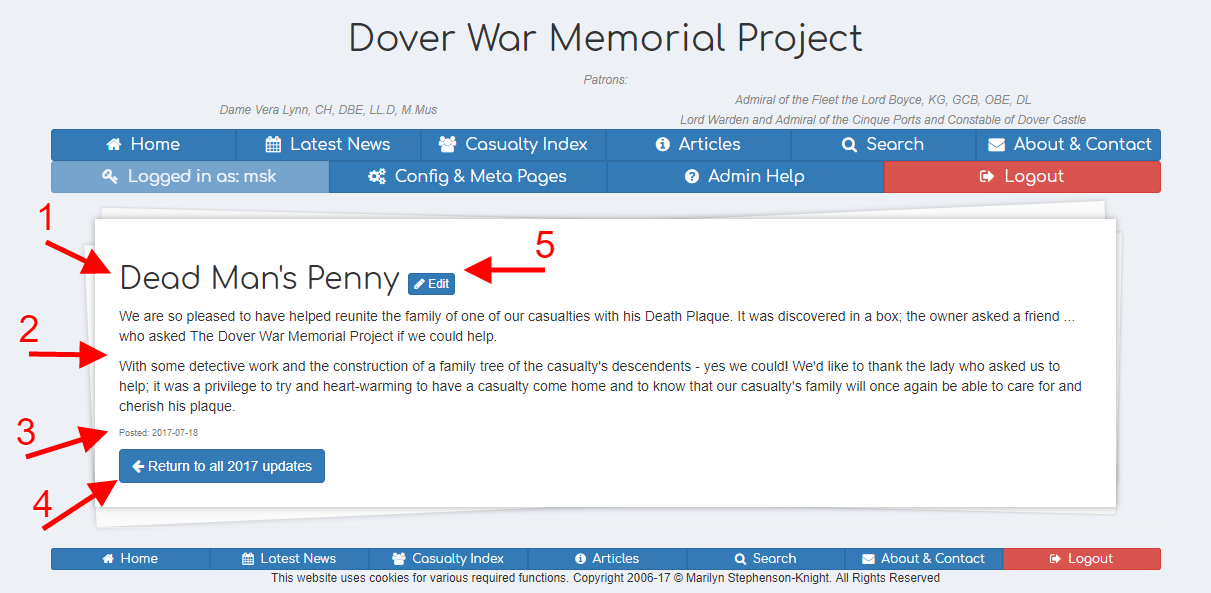
\includegraphics[width=.9\textwidth]{pics/view_update.png}
	\caption{Example of a Site Update}\label{fig:view_update}
\end{figure}

\newpage
\FloatBarrier
\subsection{How do I Add or Edit an Update?}\label{ssec:edit_update}
To create a new site update, use the \textit{Add} button on the list of updates (\marker{8}\ of Figure~\myref{fig:view_updates}. To edit an update, click the \textit{Edit} button next to the title of the update, either on the list of updates (\marker{7}\ on Figure~\myref{fig:view_updates}) or the page of a particular update (\marker{5}\ on Figure~\myref{fig:view_update}). Both methods will load a similar page, with the difference being that an Edit page will have boxes filled with data, as can be seen in Figure~\myref{fig:edit_update}.

\begin{figure}[h]
  \centering
 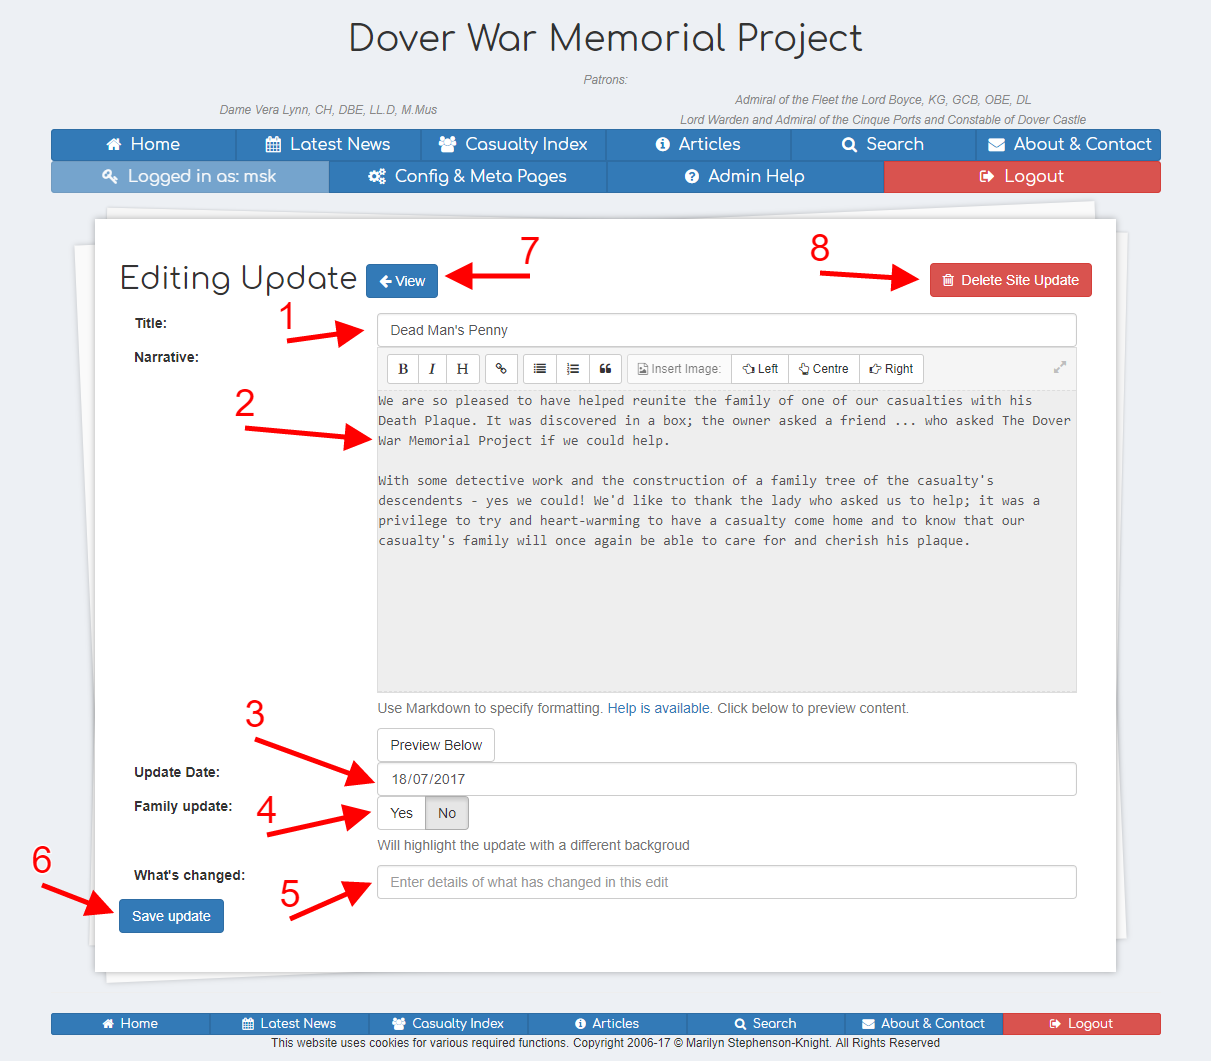
\includegraphics[width=.9\textwidth]{pics/edit_update.png}
	\caption{Example of Editing a Site Update}\label{fig:edit_update}
\end{figure}

\marker{1}\ allows the editing of the title of the site update, while \marker{2}\ allows the editing of the main content of the update. An explanation of the buttons around this area is described in Section~\myref{ssec:narrative}. \marker{3}\ shows the date this update was posted on. It is possible to set this in the future - if this is done, the update will not appear in list of updates until this date (for example, you could create a Christmas message that appears on the 25th December, without needing to log on then). A list of future updates is described in Section~\myref{ssec:config}.

\begin{infoBox}
The \texttt{title}, \texttt{content} and \texttt{date posted} fields must all be complete before the site update can be saved
\end{infoBox}

\marker{4}\ will show a slightly different background is this is a ``family update'' in a similar manner to the existing site. \marker{5}\ allows this edit to be recorded in the Change Log, if completed. Creating a new update, or substantially editing one, may be of interest so this field can be completed. For fixing a small typo, it is probably not worth it. \marker{6}\ saves this update, while \marker{7}\ returns to view this update, discarding any changes. \marker{8}\ allows the deletion of an update and is described in Section~\myref{ssec:delete_update}. The \textit{View} and \textit{Delete} buttons are not shown if this is a new memorial.

\FloatBarrier
\subsection{How do I delete an Update?}\label{ssec:delete_update}
To delete an update, navigate to its edit page, as described in Section~\myref{ssec:edit_update}. Using the \textit{Delete Site Update} button (\marker{8}\ in Figure~\myref{fig:edit_update}), will display a warning message similar to Figure~\myref{fig:delete_update}. Clicking on \textit{Cancel} (\marker{1}) will ignore this message, while \marker{2}\ will delete the site update.

\begin{warningBox}
Deletions cannot be undone
\end{warningBox}

\begin{figure}[h]
  \centering
 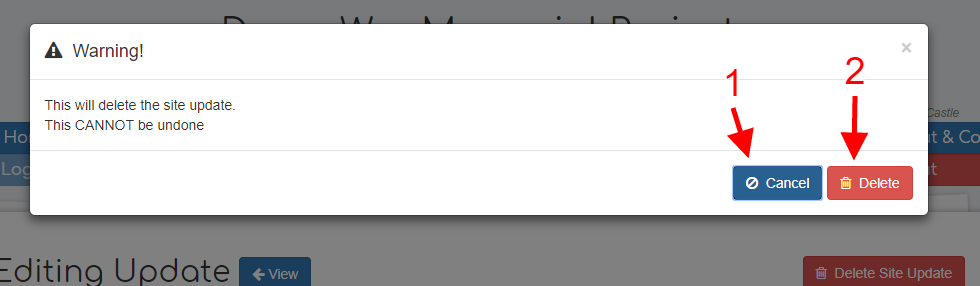
\includegraphics[width=.9\textwidth]{pics/delete_update.png}
	\caption{Deleting a Site Update}\label{fig:delete_update}
\end{figure}

\newpage
\FloatBarrier
\subsection{How do I view a List of Changes?}\label{ssec:changeLog}
To view the change log, navigate to the list of site updates (see Section~\myref{ssec:view_updates}) and click on the \textit{View change log} button, as shown by \marker{2}\ in Figure~\myref{fig:view_updates}. A page should load similar to Figure~\myref{fig:view_changes}.

\begin{figure}[h]
  \centering
 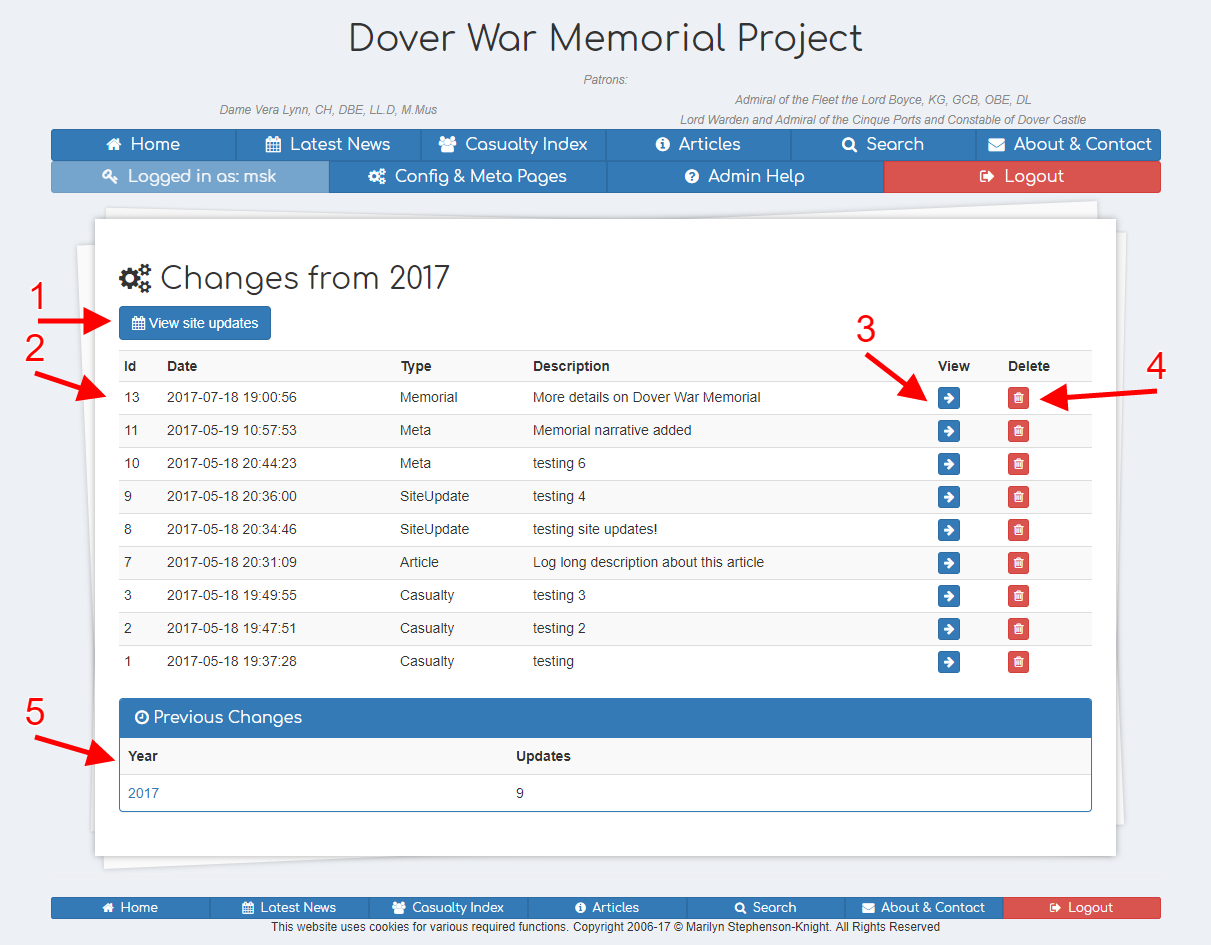
\includegraphics[width=.9\textwidth]{pics/view_changes.png}
	\caption{View the Change Log}\label{fig:view_changes}
\end{figure}

\marker{1}\ allows the user to return to the list of site updates (see Section~\myref{ssec:view_updates}). The table shown by \marker{2}\ lists the date of the change, the type of change, and the description entered. \marker{3} allows the quick navigation to the item changed, while \marker{4}\ allows the deletion of a change log item (see Section~\myref{ssec:delete_change}). \marker{5}\ indicates a summary of previous years' change log items, allowing a user to view a list of changes in the past.

\newpage
\FloatBarrier
\subsection{How do I delete an Change Log item?}\label{ssec:delete_change}
Navigate to the change log as described in Section~\myref{ssec:changeLog}. Next to the item in question, press the delete button (\marker{4} in Figure~\myref{fig:view_changes}). A panel should appear similar to Figure~\myref{fig:delete_change}. Clicking on \textit{Cancel} (\marker{1}) will ignore this message, while \marker{2}\ will delete the change log entry.

\begin{warningBox}
Deletions cannot be undone
\end{warningBox}

\begin{figure}[h]
  \centering
 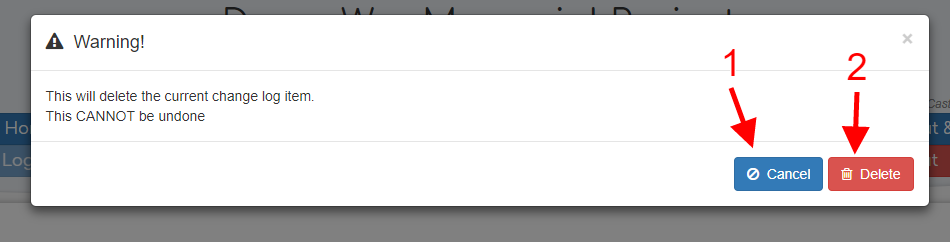
\includegraphics[width=.9\textwidth]{pics/delete_change.png}
	\caption{Deleting a Change Log Entry}\label{fig:delete_change}
\end{figure}

\newpage
\FloatBarrier
\section{Casualty Index}\label{sec:casualtyIndex}

The casualty index is the main section of the site, and therefore has a lot of details associated with it. Casualties are grouped into one or more memorials, with a few main ones shown in more prominence on the main memorial list (the same ones that are shown on the old site). Lists of casualties are displayed on each memorial's page. There is also a memorial map, which shows the various memorials on a interactive map. A casualty as the same narrative before, along with their pictures, as well as a section full of data - used to create the relational and searchable database.

\subsection{How do I view a List of all Memorials?}\label{ssec:view_memorials}
Navigate to the list of memorials by clicking the \textit{Casualty Index} button on the top or bottom menu bar. A page should load similar to Figure~\myref{fig:view_memorials}.

\begin{figure}[h]
  \centering
 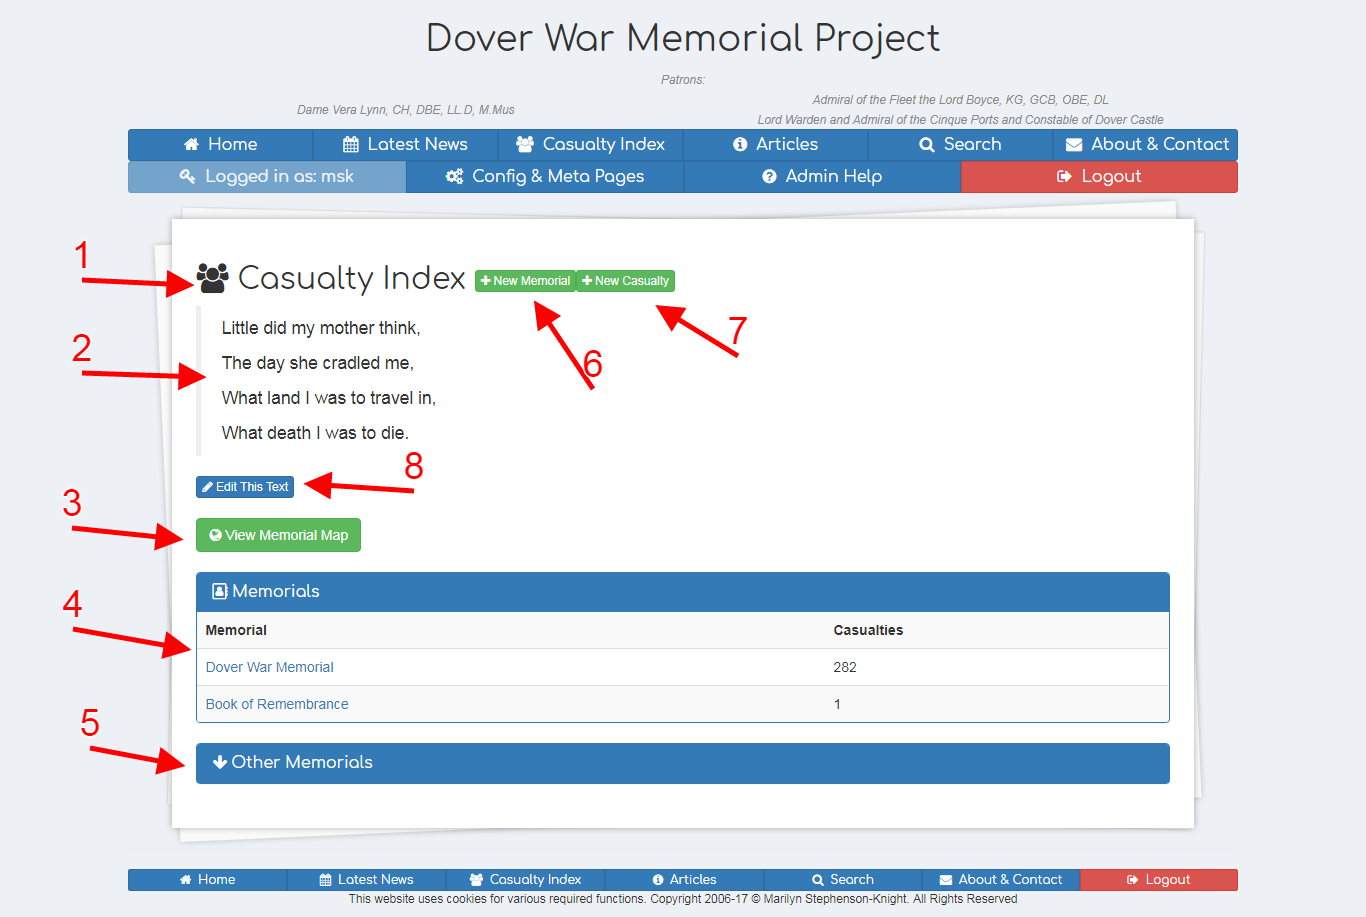
\includegraphics[width=.9\textwidth]{pics/view_memorials.png}
	\caption{View the List of Memorials}\label{fig:view_memorials}
\end{figure}

\marker{1}\ shows the title of the page, while \marker{2}\ provides some narrative content (which can be edited using \marker{8}). \marker{3}\ links to the memorial map, while the list of memorials are indicated by \marker{4}\. the name of the memorial and the number of casualties are shown. \marker{5}\ allows the user to also view the other memorials, which are displayed in the same way. \marker{6}\ and \marker{7}\ allow the creation of a new memorial and casualty respectively.

\newpage
\FloatBarrier
\subsection{How do I view the Memorial Map?}
To view the memorial map, navigate to the list of memorials (see Section~\myref{ssec:view_memorials}) and click on the \textit{Memorial Map} button, as shown by \marker{3}\ in Figure~\myref{fig:view_memorials}. A page should load similar to Figure~\myref{fig:view_map}.

\begin{figure}[h]
  \centering
 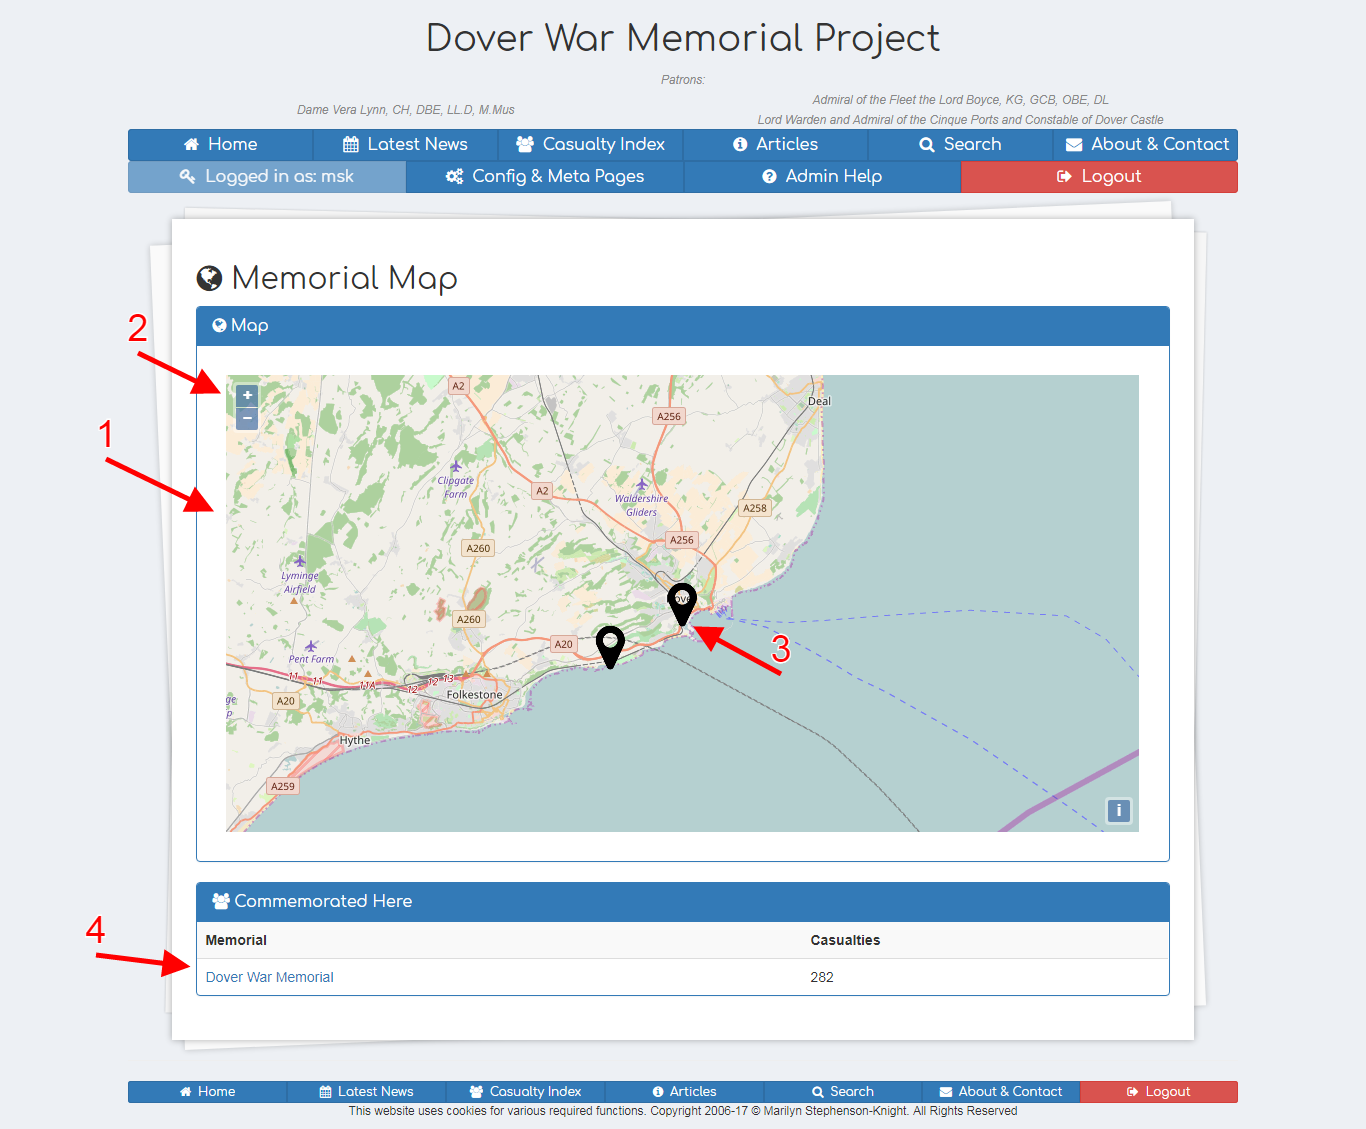
\includegraphics[width=.9\textwidth]{pics/view_map.png}
	\caption{View the Memorial Map}\label{fig:view_map}
\end{figure}

The main map window is shown in \marker{1}\ with some navigation buttons displayed in \marker{2}. The map uses standard navigation features: dragging, scrolling, etc. Clicking on a black pin, as indicated by \marker{3}, will show a panel below (\marker{4}) detailing the name and number of casualties at that memorial.
\begin{infoBox}
Only memorials with latitude and longitude information are displayed on this map, and by default, it will centre on Dover.
\end{infoBox}

\newpage
\FloatBarrier
\subsection{How do I view a particular Memorial?}
To view the memorial map, navigate to the list of memorials (see Section~\myref{ssec:view_memorials}) and click on the name of any memorial. A page will load similar to Figure~\myref{fig:view_memorial}.

\begin{figure}[h]
  \centering
 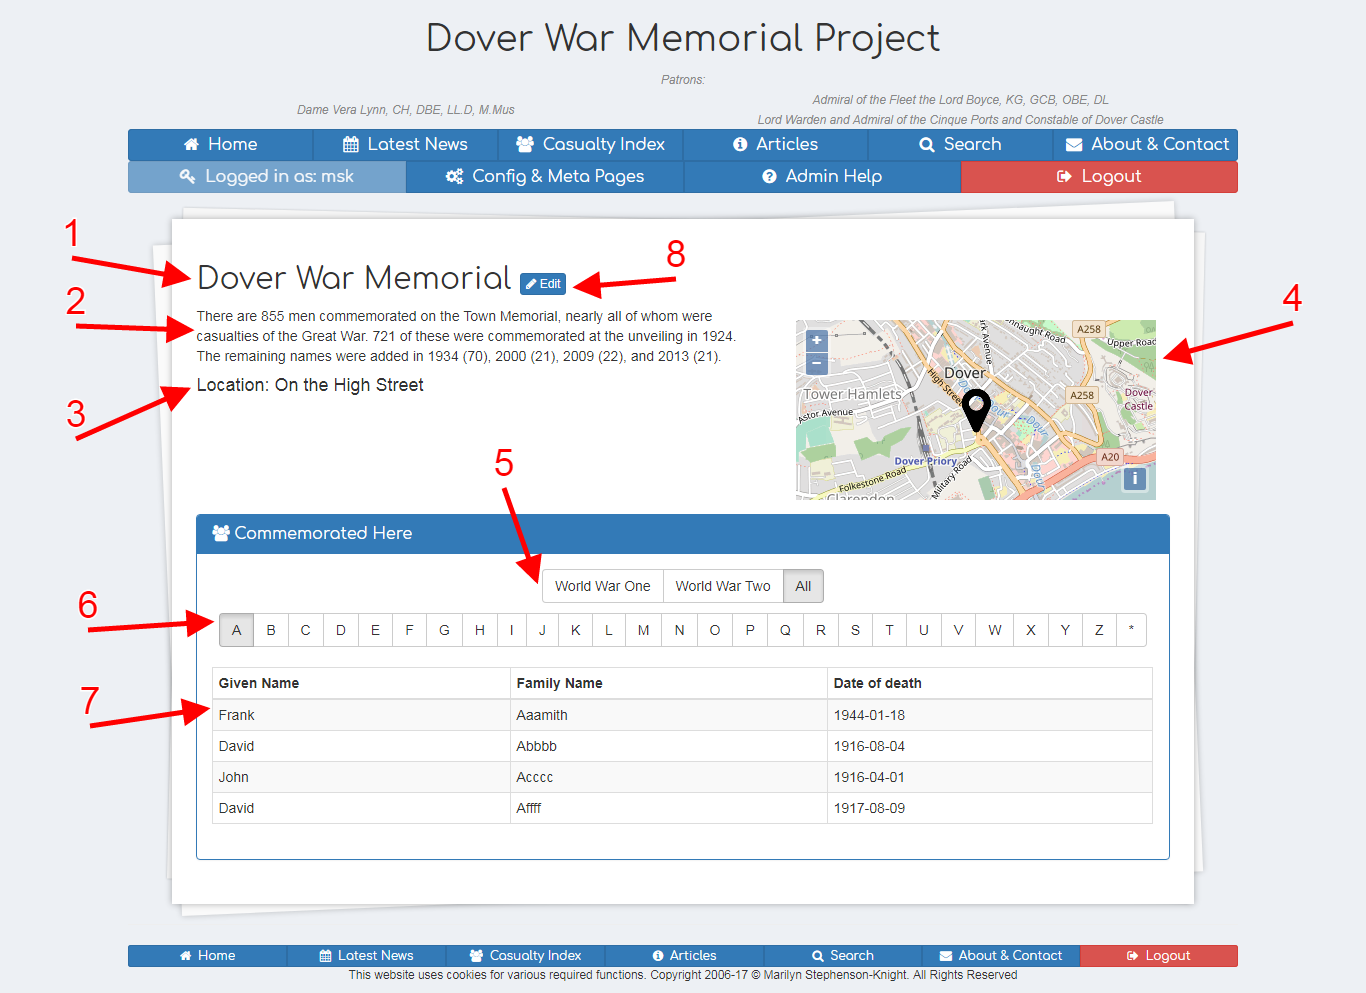
\includegraphics[width=.9\textwidth]{pics/view_memorial.png}
	\caption{View a particular memorial}\label{fig:view_memorial}
\end{figure}

\marker{1}\ gives the title of the memorial, while \marker{2}\ displays the narrative content, editable using the button indicated by \marker{8}. A text description of the location is shown by \marker{3}\ (for example, if the memorial is a book, or perhaps a grave reference number), with a map shown by \marker{4}. \marker{5}\ allows the user to filter casualties by the two World Wars, or by all wars, while \marker{6}\ allows the filtering by surname. The list of filtered casualties is indicated by \marker{7} and navigates to that casualty's particular page.

\begin{infoBox}
If no latitude or longitude has been set then the map is not displayed.
\end{infoBox}

\newpage
\FloatBarrier
\subsection{How do I Add or Edit a Memorial?}\label{ssec:edit_memorial}
To create a new memorial, use the \textit{New Memorial} button on the list of memorials (\marker{6}\ of Figure~\myref{fig:view_memorials}). To edit an update, click the \textit{Edit} button next to the title of the memorial on the page of a particular memorial (\marker{8}\ on Figure~\myref{fig:view_memorial}). Both methods will load a similar page, with the difference being that an Edit page will have boxes filled with data, as can be seen in Figure~\myref{fig:edit_memorial}.

\begin{figure}[h]
  \centering
 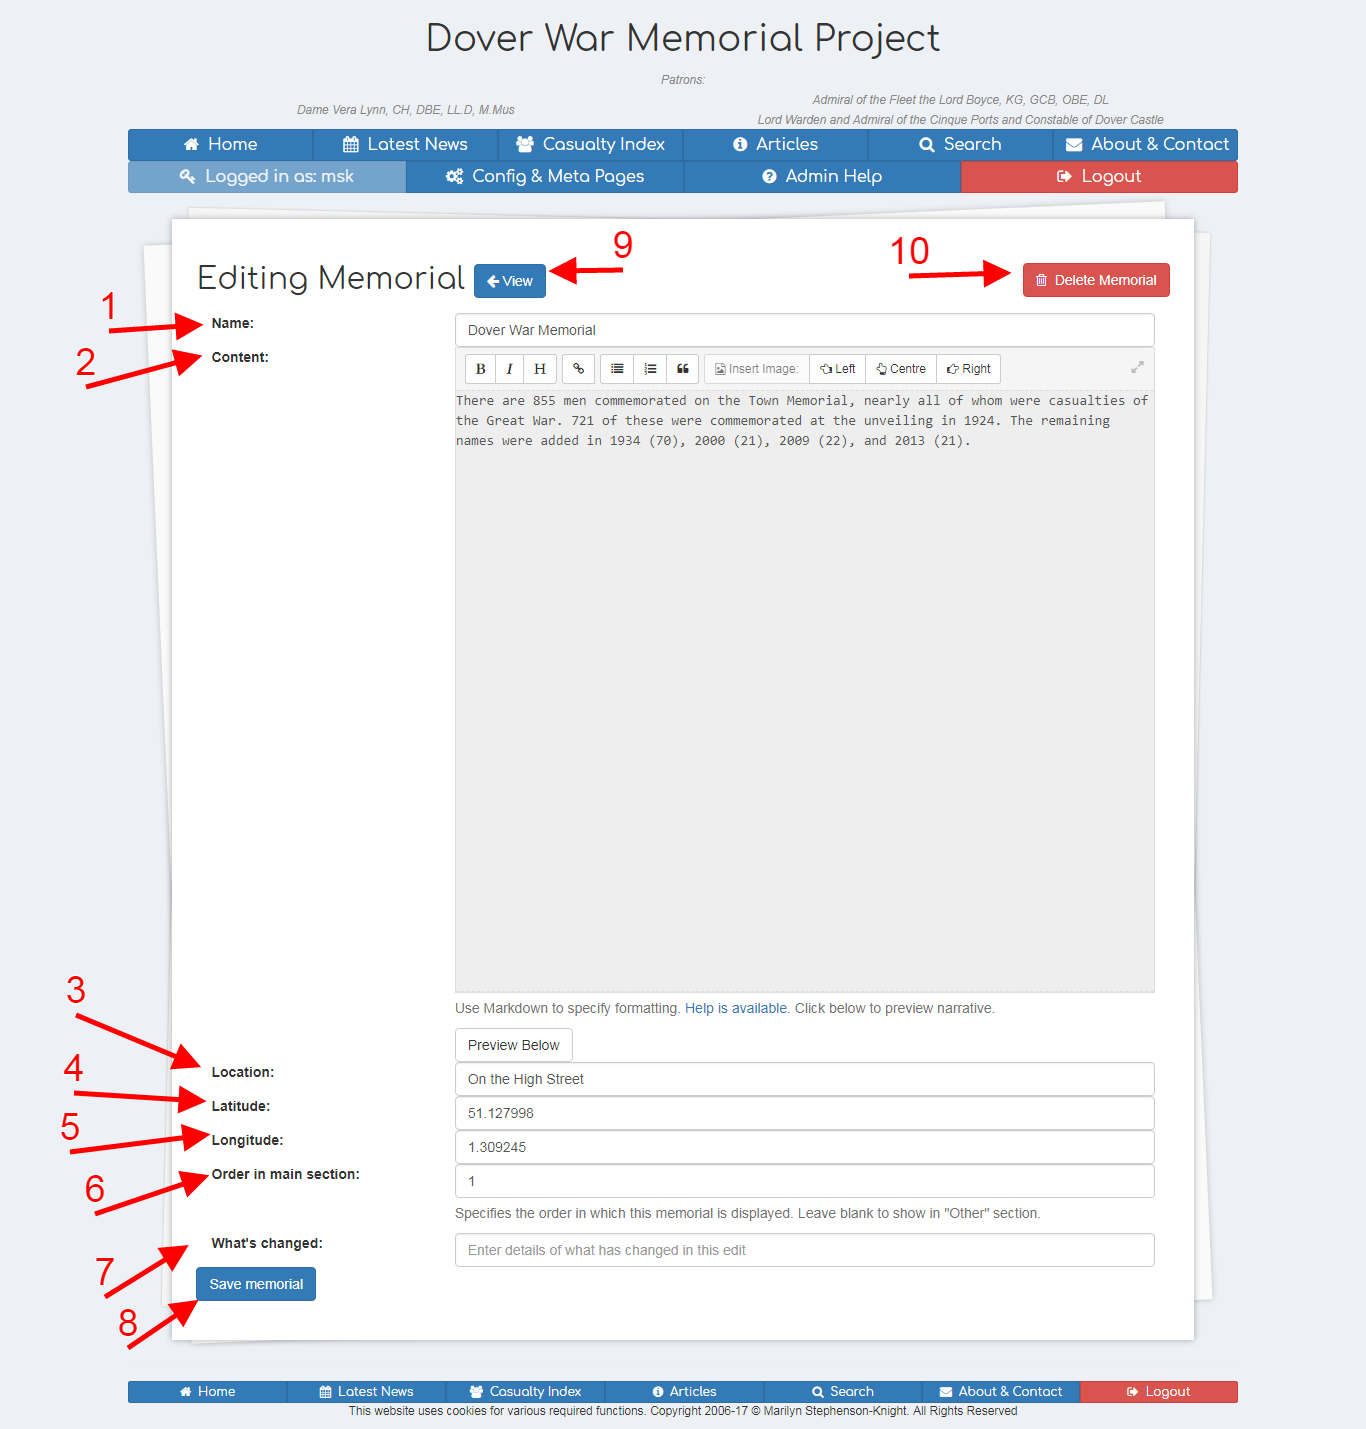
\includegraphics[width=.9\textwidth]{pics/edit_memorial.png}
	\caption{Editing a Memorial}\label{fig:edit_memorial}
\end{figure}

\marker{1}\ indicates the name of the memorial, with \marker{2}\ indicating the narrative content. An explanation of the buttons around this area is described in Section~\myref{ssec:narrative}. \marker{4}\ indicates the text description of the location of the memorial, while \marker{4}\ and \marker{5}\ contain the latitude and longitude (as decimal numbers). 

\begin{infoBox}
On Google Maps, right click and select \textit{What's here?}. At the bottom of the screen, the latitude and longitude of the clicked location is shown.
\end{infoBox}

\marker{6}\ indicates the order in which this memorial should appear in the main list of memorials. If this memorial should not appear in the main list, then leave this blank. The lower a number, the higher it will be displayed on the list. \marker{7}\ allows this edit to be recorded in the Change Log, if completed. Creating a new update, or substantially editing one, may be of interest so this field can be completed. For fixing a small typo, it is probably not worth it. \marker{8}\ saves this memorial, while \marker{9}\ returns to view this memorial, discarding any changes. \marker{10}\ allows the deletion of an update and is described in Section~\myref{ssec:delete_memorial}. The \textit{View} and \textit{Delete} buttons are not shown if this is a new memorial.

\begin{infoBox}
The \texttt{name} and \texttt{content} fields must all be complete before the site update can be saved
\end{infoBox}

\FloatBarrier
\subsection{How do I delete a Memorial?}\label{ssec:delete_memorial}
To delete a memorial, navigate to its edit page, as described in Section~\myref{ssec:edit_memorial}. Using the \textit{Delete Memorial} button (\marker{10}\ in Figure~\myref{fig:edit_memorial}), will display a warning message similar to Figure~\myref{fig:delete_memorial}. Clicking on \textit{Cancel} (\marker{1}) will ignore this message, while \marker{2}\ will delete the memorial.

\begin{warningBox}
Any casualties with this memorial will have it removed. This may mean some casualties have no memorial and therefore will be displayed in a list as described in Section~\myref{ssec:config}.\\
Deletions cannot be undone
\end{warningBox}

\begin{figure}[h]
  \centering
 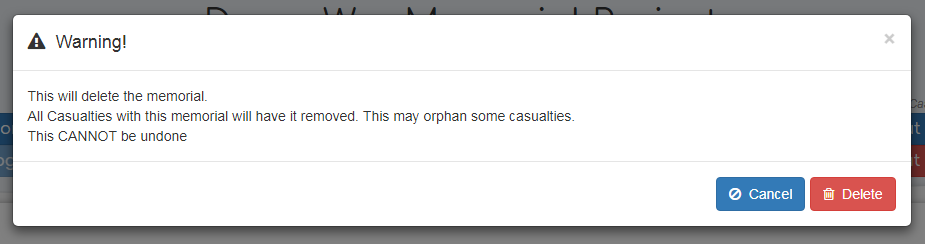
\includegraphics[width=.9\textwidth]{pics/delete_memorial.png}
	\caption{Deleting a Memorial}\label{fig:delete_memorial}
\end{figure}

\newpage
\FloatBarrier
\subsection{How do I view a Casualty?}\label{ssec:view_casualty}
To navigate to a particular casualty, navigate to a particular memorial and choose the casualty from the list (\marker{7}\ from Figure~\myref{fig:view_memorial}). It is also possible to arrive at a casualty from the home page if they are commemorated on this particular date. A page should load similar to Figure~\myref{fig:view_casualty}.

\begin{figure}[h]
  \centering
 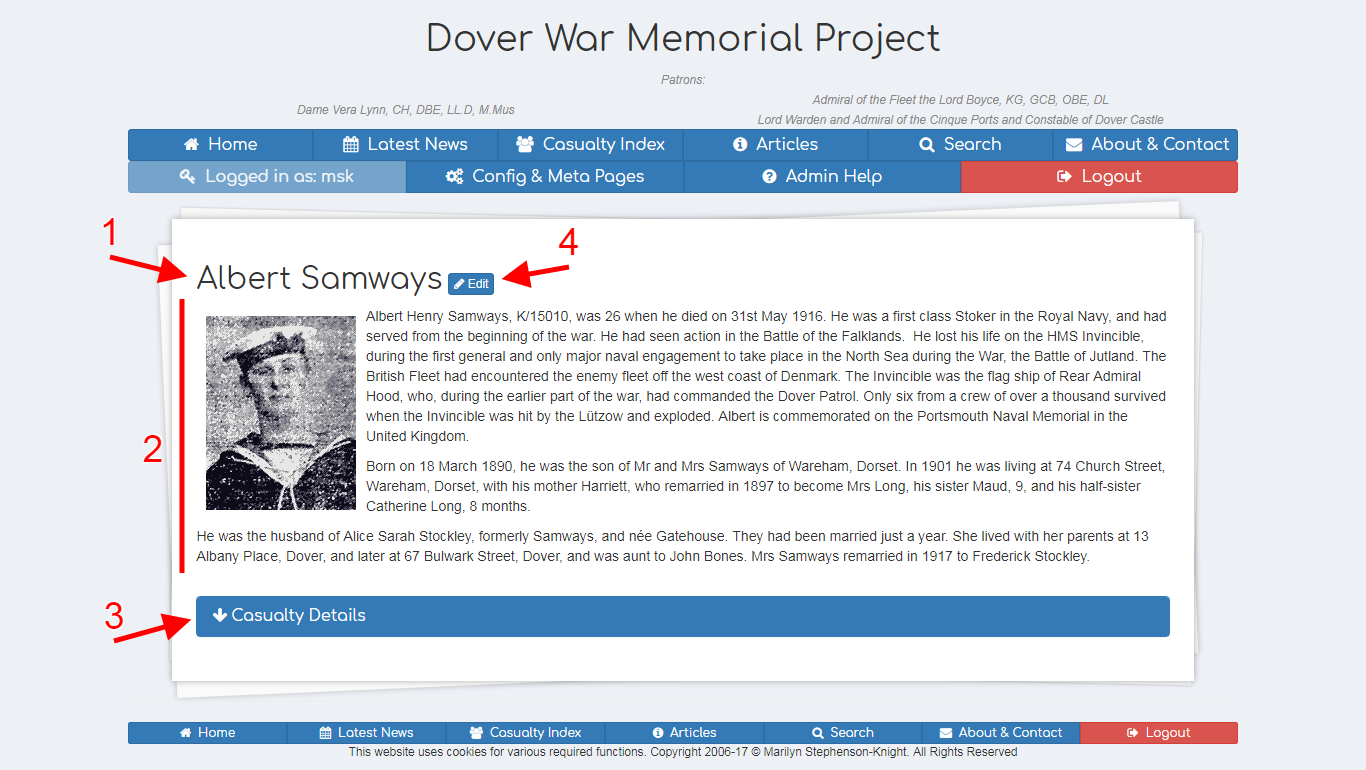
\includegraphics[width=.9\textwidth]{pics/view_casualty.png}
	\caption{Viewing a Casualty}\label{fig:view_casualty}
\end{figure}

\marker{1}\ indicates the name of this casualty (their given name and family name). \marker{2}\ indicates the main narrative section of the casualty, including any pictures. \marker{3}\ shows the data for the particular casualty, while \marker{4} indicates a button that allows the editing of this casualty (see Section~\myref{ssec:edit_casualty}).

\newpage
\FloatBarrier
\subsection{How do I view a Casualty's Data?}\label{ssec:view_casualty_data}
Clicking on \marker{3}\ on Figure~\myref{fig:view_casualty} will adjust the page to show the full data of this casualty, as shown in Figure~\myref{fig:view_casualty_data}.

\begin{figure}[h]
  \centering
 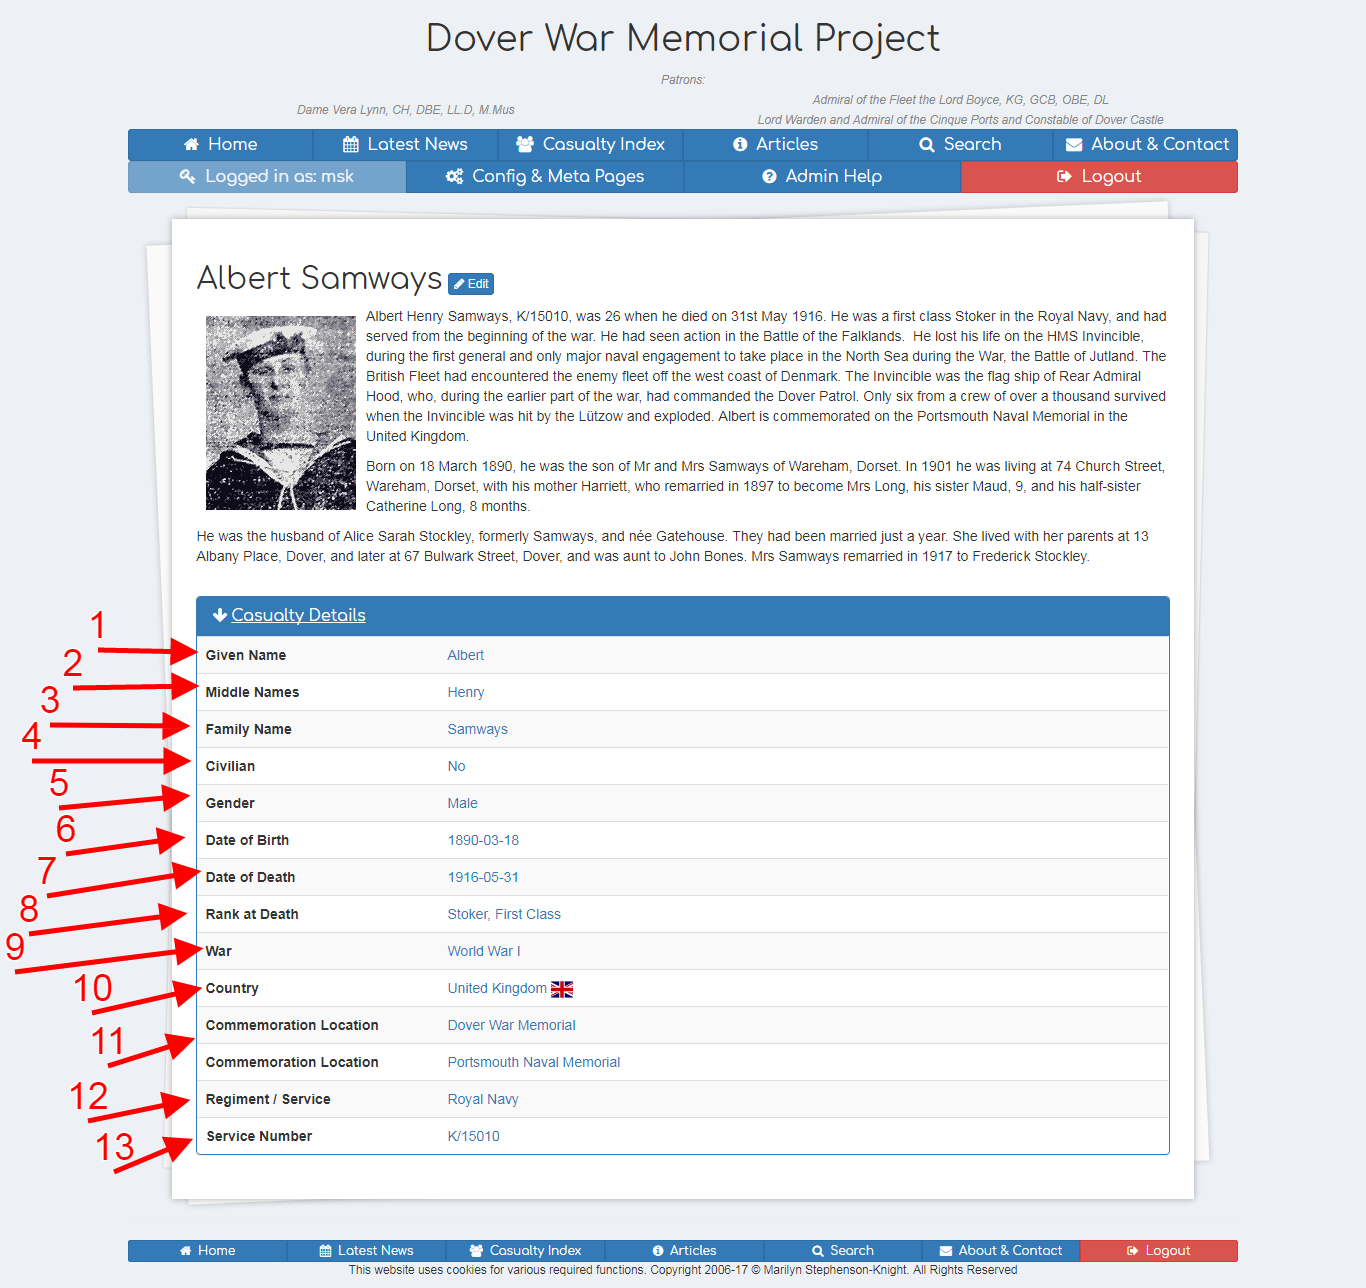
\includegraphics[width=.9\textwidth]{pics/view_casualty_data.png}
	\caption{Viewing a Casualty}\label{fig:view_casualty_data}
\end{figure}

\marker{1}, \marker{2}\ and \marker{3}\ all indicate the full name of the given casualty, while \marker{4}\ indicates if they are a civilian. \marker{5}\ indicates their gender and \marker{6}\ and \marker{7}\ indicate the casualty's date of birth and death respectively. \marker{8}\ indicates their rank at death, while \marker{9}\ indicates the particular war they died in. \marker{10}\ indicates the country for which they served, while \marker{11}\ shows any commemoration locations (in this example, there are two). \marker{12}\ indicates the Regiment or Service, while \marker{13}\ indicates any service numbers the casualty may have had. Any relations would be displayed below, although this casualty has none.

\begin{infoBox}
If a particular piece of data is not available, then the row will be missing.\\
Clicking on a piece of data will create a search based around it.
\end{infoBox}

\newpage
\FloatBarrier
\subsection{How do I Add or Edit a Casualty?}\label{ssec:edit_casualty}
To create a new casualty, use the \textit{Add} button on the list of memorials (\marker{7}\ of Figure~\myref{fig:view_memorials}). To edit a casualty, click the \textit{Edit} button next to the name of the casualty on the page of a particular casualty (\marker{4}\ on Figure~\myref{fig:view_casualty}). Both methods will load a similar page, with the differences being that an Edit page will have boxes filled with data and will not have a \textit{View} or \textit{Delete} button, as can be seen in Figures~\myref{fig:edit_casualty} and ~\myref{fig:edit_casualty2}.
\begin{infoBox}
The Add page will also only display the first section until the casualty is saved.
\end{infoBox}

\begin{figure}[h]
  \centering
 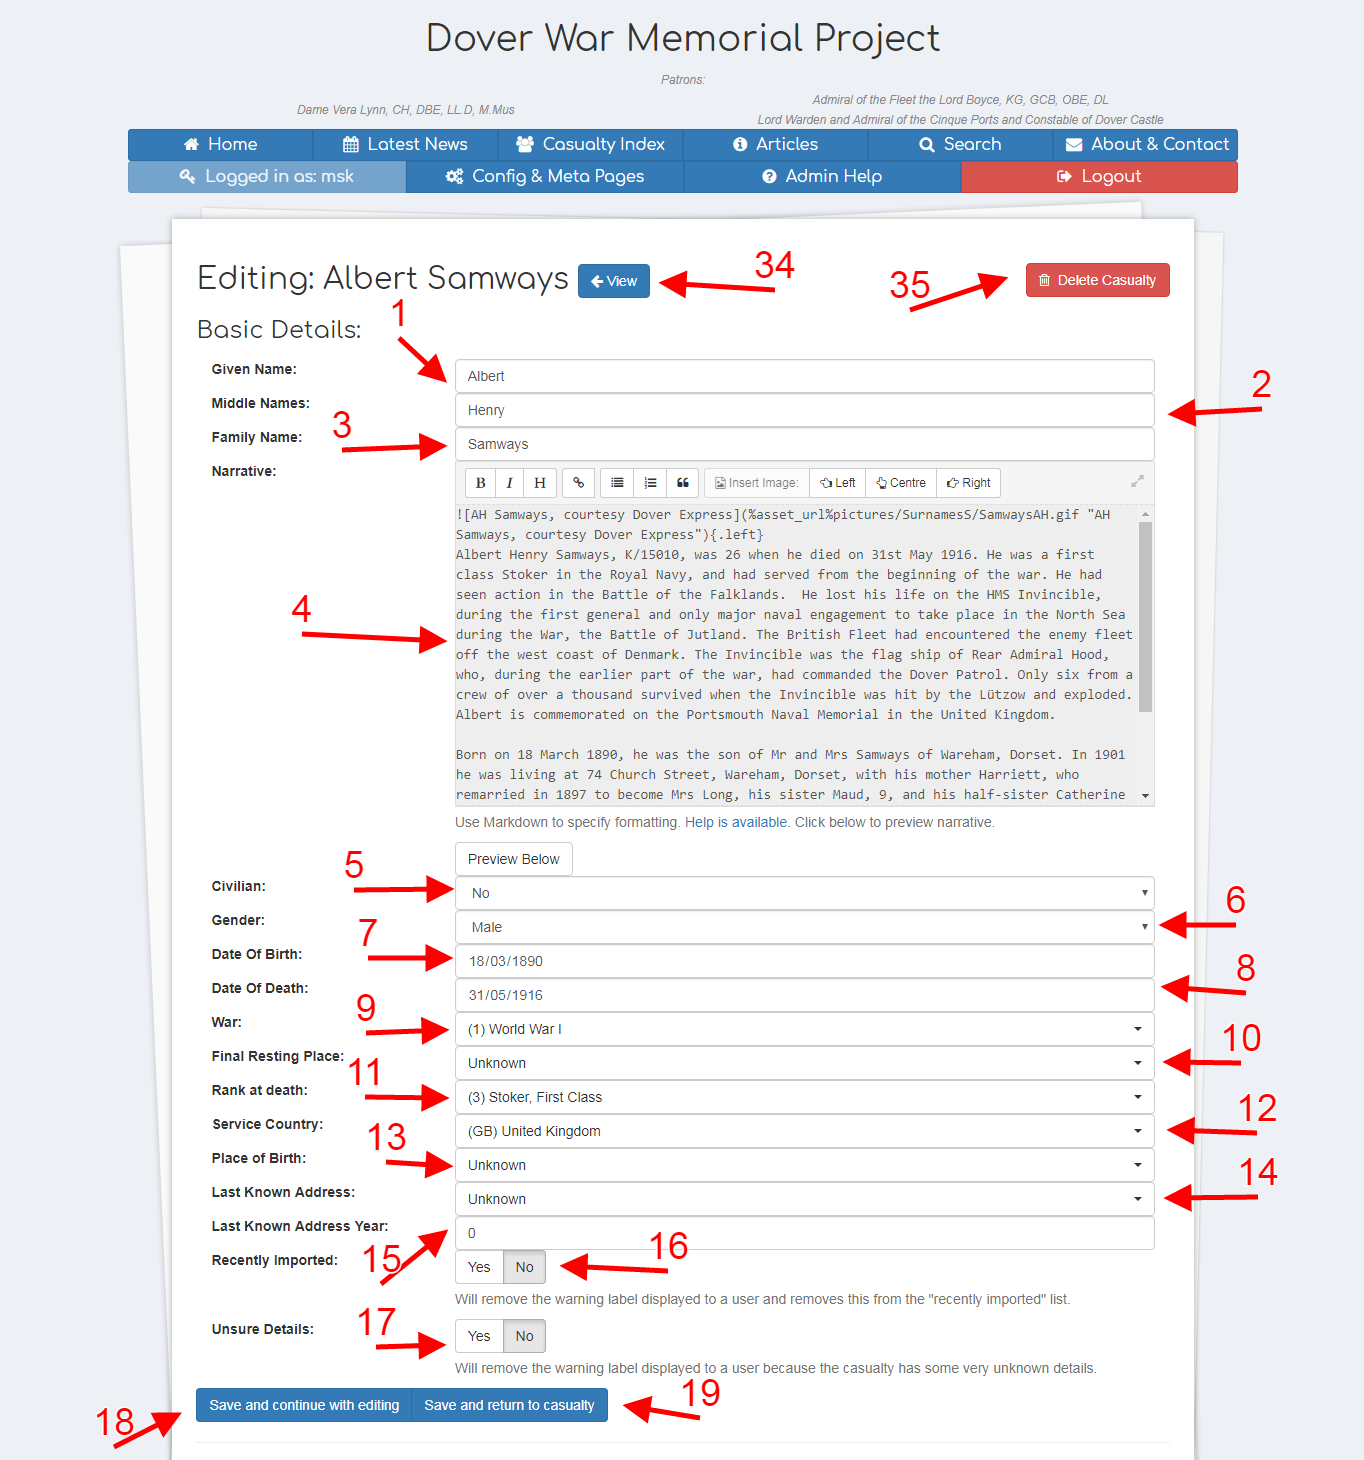
\includegraphics[width=.9\textwidth]{pics/edit_casualty.png}
	\caption{Example of Editing a Casualty (1)}\label{fig:edit_casualty}
\end{figure}
\newpage
\begin{figure}[h]
  \centering
 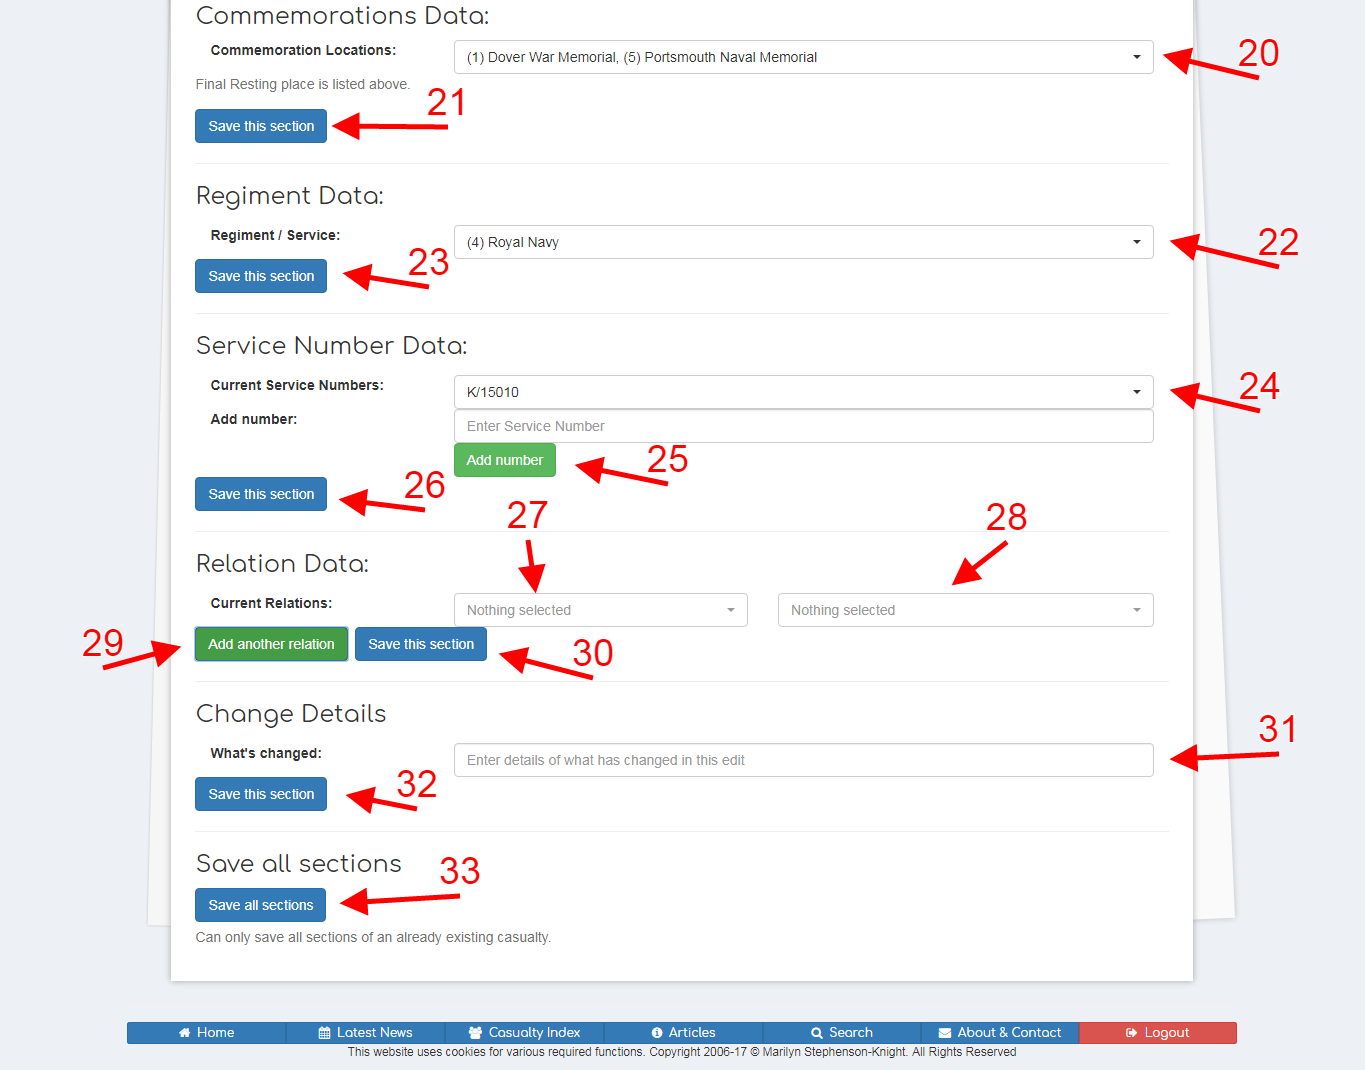
\includegraphics[width=.9\textwidth]{pics/edit_casualty2.png}
	\caption{Example of Editing a Casualty (2)}\label{fig:edit_casualty2}
\end{figure}

\marker{1}, \marker{2}\ and \marker{3}\ all indicate the full name of the given casualty, while \marker{4}\ contains the narrative content for this casualty. An explanation of the buttons around this area is described in Section~\myref{ssec:narrative}. \marker{5}\ identifies a dropdown box that allows the selection of the casualty's civilian status, while \marker{6}\ determines their gender. \marker{7}\ and \marker{8}\ indicate the casualty's date of birth and death. When hovering over these fields, a dropdown is possible that displays a calendar - this may not be too useful for the dates that are likely to be in these fields, however. Next, \marker{9}\ provides a dropdown with a list of potential wars this casualty may have died in, while \marker{10}\ allows the selection of their final resting place. \marker{12}\ provides another dropdown, this time for the service country, with \marker{13}\ allows for the selection of the casualty's place of birth. \marker{14}\ and \marker{15}\ allow for the selection of the Last Known Address and the year that it was known. \marker{16}\ indicates if this casualty was recently imported - if so, a message is displayed to the user informing that the data may not be complete. \marker{17}\ indicates if some details are unknown, and if so, a message is displayed to the user. This replaces the previous method of placing an asterisk next to a casualty's name. \marker{18}\ saves the current casualty and returns to this edit page (this must be completed when creating a new casualty for the other sections to appear), while \marker{19}\ returns to the casualty's page. \marker{34}\ returns to the casualty page without saving while \marker{35}\ deletes this casualty (as shown in Section~\myref{ssec:delete_casualty}).

\begin{infoBox}
The \texttt{name} and \texttt{content} fields must all be complete before the site update can be saved.
\end{infoBox}

\marker{20}\ allows the user to select or deselect a number of commemoration locations for this casualty, and \marker{21}\ saves this section.

\marker{22}\ allows the user to select or deselect a number of Regiments (use this section for regiments, services (Army, Navy etc), ships and so on) for this casualty, and \marker{23}\ saves this section.

\marker{24}\ allows the user to select or deselect a number of existing service numbers for this casualty. To add a new number to list list, type in the empty box. \marker{25}\ allows extra boxes to be added if needed. \marker{26}\ saves this section.

The next section allows relation data to be added. This indicates that casualties were family members. Select a casualty using the dropdown indicated by \marker{27}\ and the relation type indicated by \marker{28}. To remove a relation, simply set both boxes to be empty. \marker{29}\ allows more relations to be added and \marker{30}\ saves this section.

\marker{31}\ allows this edit to be recorded in the Change Log, if completed. Creating a new update, or substantially editing one, may be of interest so this field can be completed. For fixing a small typo, it is probably not worth it.

\marker{33}\ saves all the sections on this page.

\begin{infoBox}
Many dropdowns allow searching. Type to limit the results shown. \\
Clicking on a selected choice will deselect it.
\end{infoBox}

\FloatBarrier
\subsection{How do I delete a Casualty?}\label{ssec:delete_casualty}
To delete a casualty, navigate to its edit page, as described in Section~\myref{ssec:edit_casualty}. Using the \textit{Delete Casualty} button (\marker{35}\ in Figure~\myref{fig:edit_casualty}), will display a warning message similar to Figure~\myref{fig:delete_casualty}. Clicking on \textit{Cancel} (\marker{1}) will ignore this message, while \marker{2}\ will delete the casualty.

\begin{warningBox}
Deletions cannot be undone
\end{warningBox}

\begin{figure}[h]
  \centering
 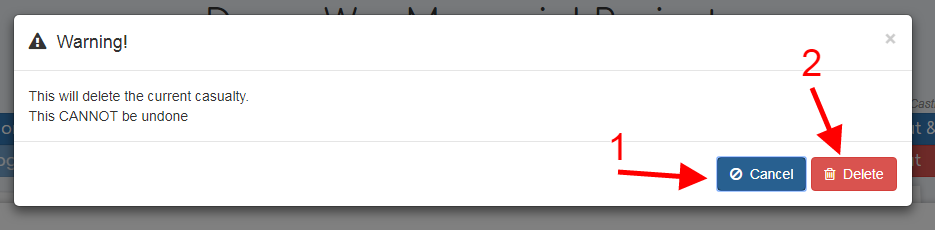
\includegraphics[width=.9\textwidth]{pics/delete_casualty.png}
	\caption{Deleting a Casualty}\label{fig:delete_casualty}
\end{figure}

\newpage
\FloatBarrier
\section{Articles}\label{sec:articles}
The articles section is the same as the Information Index on the old site. The renaming is mainly because ``Information Index'' doesn't fit into the menu bars, and is a bit snappier.

Information that was on other areas of the site (e.g. the article about the Dover War Memorial, Donate, etc) should be classed as an article, but won't belong in one of the groups that existed on the previous site, and therefore won't be listed on the main Articles page. There is a separate list (see Section~\myref{ssec:config}) of Articles which do not belong in any category.

\subsection{How do I view the list of Articles?}\label{ssec:view_articles}
Navigate to the list of articles by clicking the \textit{Articles} button on the top or bottom menu bar. A page should load similar to Figure~\myref{fig:view_articles}.

\begin{figure}[h]
  \centering
 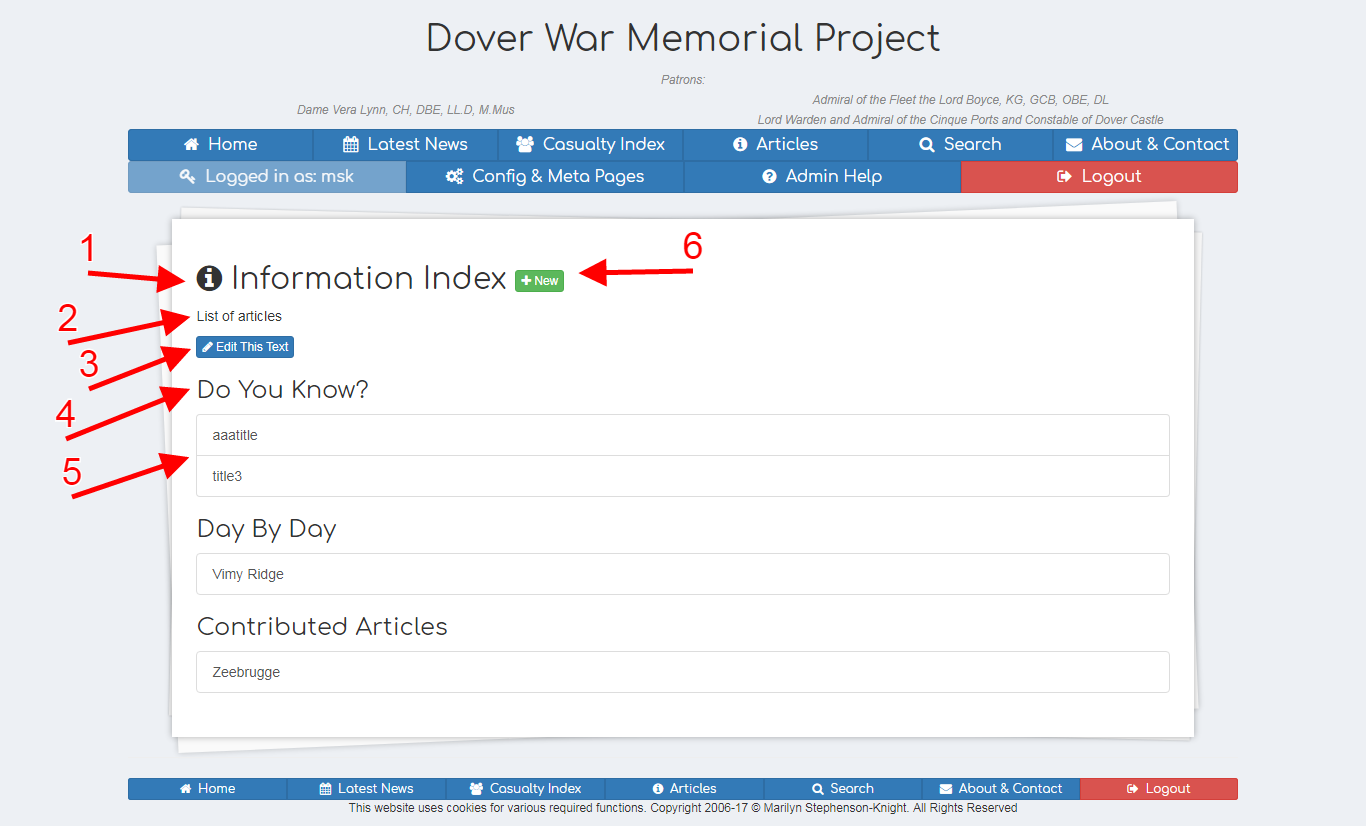
\includegraphics[width=.9\textwidth]{pics/view_articles.png}
	\caption{View List of Articles}\label{fig:view_articles}
\end{figure}

\marker{1}\ is the title of the page - this one says Information Index. \marker{2}\ contains some narrative about the list of articles, while \marker{3}\ allows the user to edit this text. \marker{4}\ indicates the title of each category, while \marker{5} shows the list of articles in each category.

\begin{infoBox}
If there are no articles in a category, it is not shown.
\end{infoBox}

\newpage
\FloatBarrier
\subsection{How do I view a particular Article?}\label{ssec:view_article}
To view a particular article, click on the title of that article in the list of articles (see Section~\myref{ssec:view_articles}). A page will load similar to Figure~\myref{fig:view_article}.

\begin{figure}[h]
  \centering
 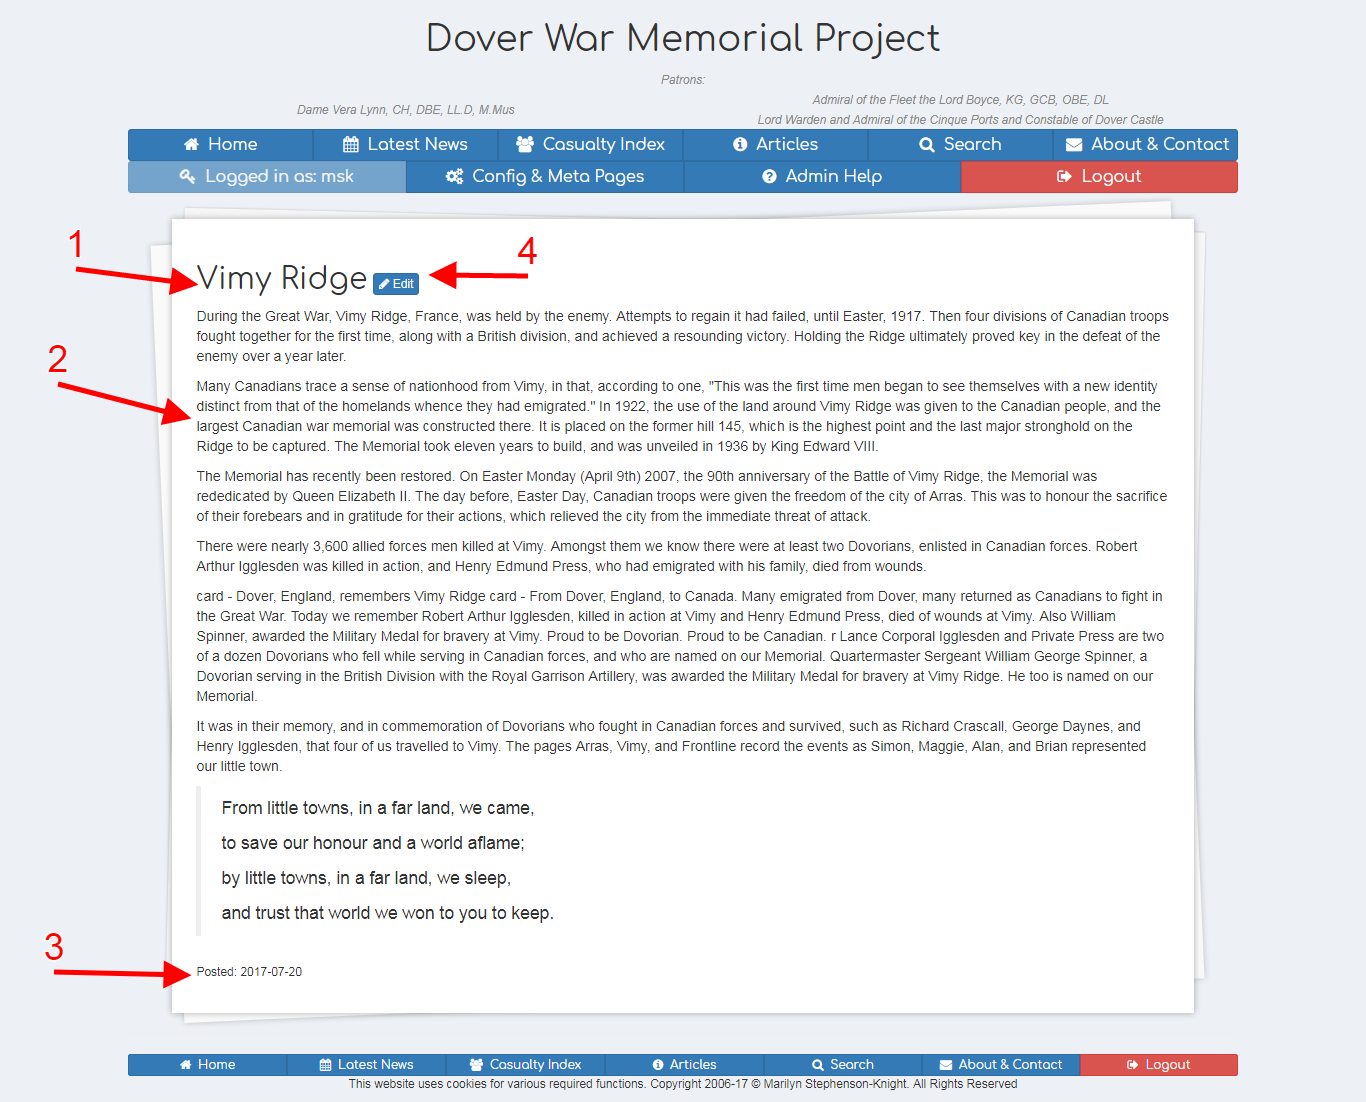
\includegraphics[width=.9\textwidth]{pics/view_article.png}
	\caption{View a particular Article}\label{fig:view_article}
\end{figure}

\marker{1}\ indicates the title of the article, while \marker{2}\ indicates the narrative content. \marker{3}\ shows the date the article was posted, while \marker{4}\ indicates a button to edit the article (see Section~\myref{ssec:edit_article}).

\newpage
\FloatBarrier
\subsection{How do I Add or Edit an Article?}\label{ssec:edit_article}
To create a new article, use the \textit{Add} button on the list of articles (\marker{6}\ of Figure~\myref{fig:view_articles}). To edit an article, click the \textit{Edit} button next to the title of the article (\marker{4}\ on Figure~\myref{fig:view_article}). Both methods will load a similar page, with the differences being that an Edit page will have boxes filled with data and will not have a \textit{View} or \textit{Delete} button, as can be seen in Figure~\myref{fig:edit_article}.

\begin{figure}[h]
  \centering
 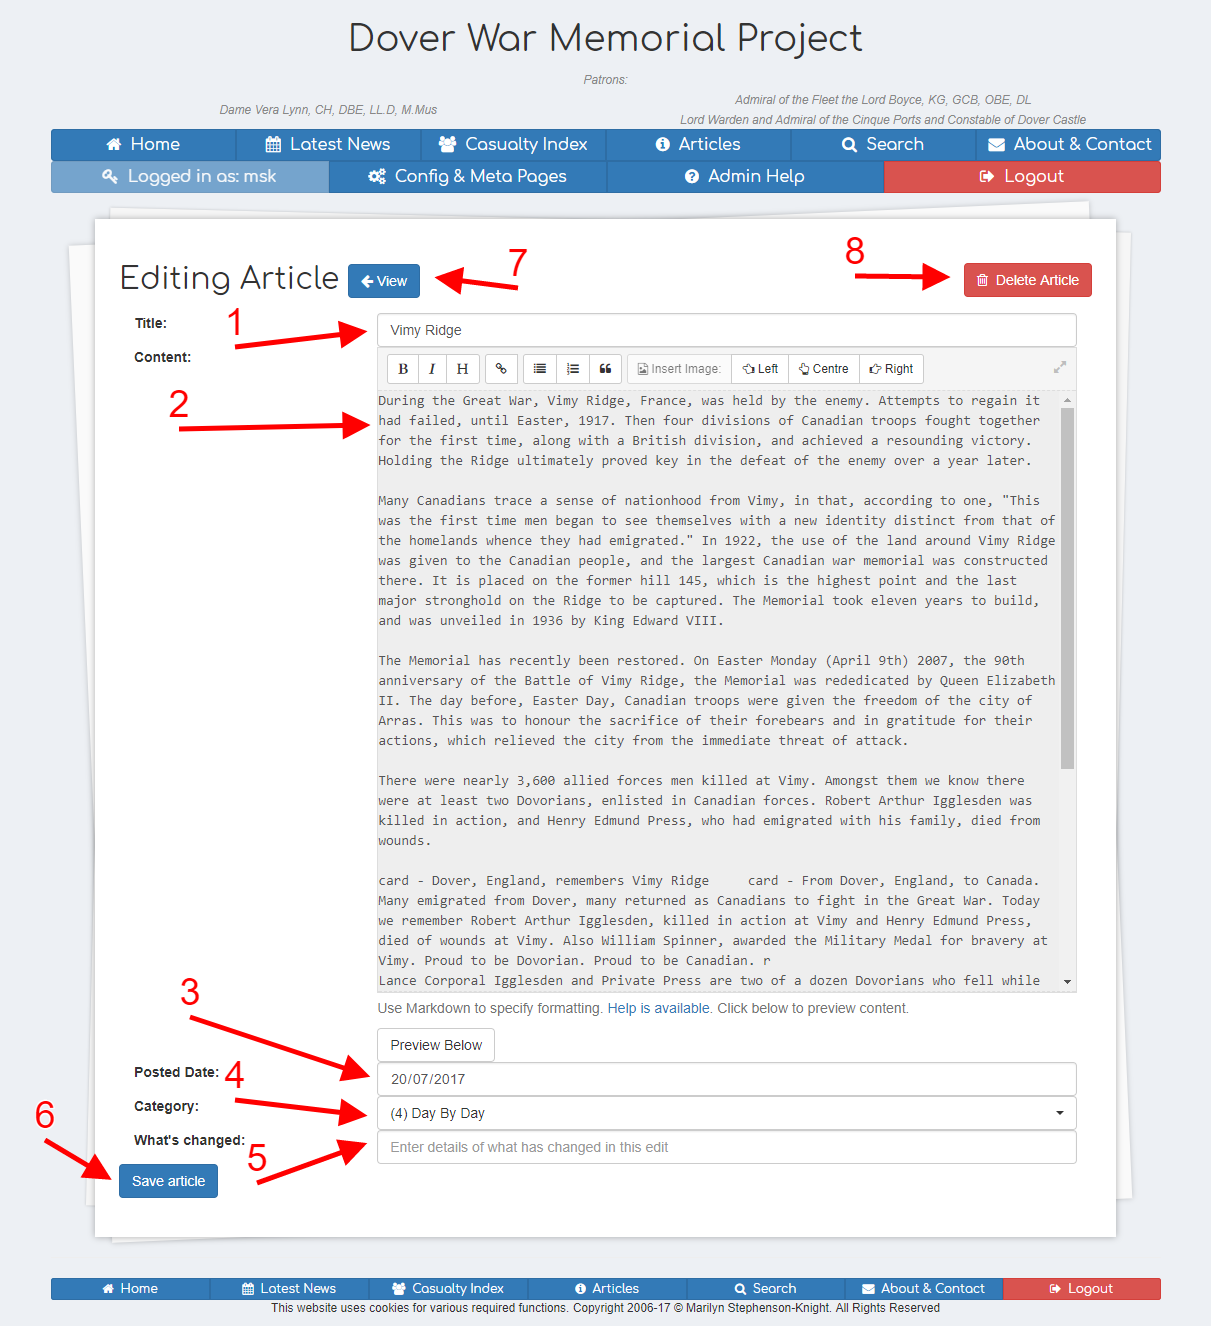
\includegraphics[width=.9\textwidth]{pics/edit_article.png}
	\caption{Example of Editing an Article}\label{fig:edit_article}
\end{figure}

\marker{1}\ indicates the title of the article, while \marker{2}\ contains the narrative content for this article. An explanation of the buttons around this area is described in Section~\myref{ssec:narrative}. The date the article was posted is shown by \marker{3}\ and the category by \marker{4}. If no category is specified, the article will not appear on the Information Index, but may be linked to from elsewhere. \marker{5}\ allows this edit to be recorded in the Change Log, if completed. Creating a new update, or substantially editing one, may be of interest so this field can be completed. For fixing a small typo, it is probably not worth it. \marker{6}\ saves the changes to the article, while \marker{7}\ returns to view the article with the changes unsaved. \marker{8} allows the deletion of this article, as described in Section~\myref{ssec:delete_article}.

\FloatBarrier
\subsection{How do I delete an Article?}\label{ssec:delete_article}

To delete an article, navigate to its edit page, as described in Section~\myref{ssec:edit_article}. Using the \textit{Delete Article} button (\marker{8}\ in Figure~\myref{fig:edit_article}), will display a warning message similar to Figure~\myref{fig:delete_article}. Clicking on \textit{Cancel} (\marker{1}) will ignore this message, while \marker{2}\ will delete the article.

\begin{warningBox}
Deletions cannot be undone
\end{warningBox}

\begin{figure}[h]
  \centering
 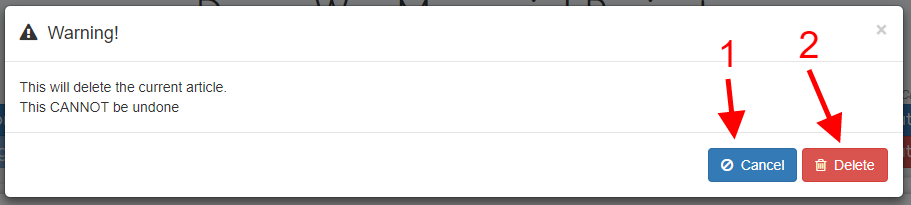
\includegraphics[width=.9\textwidth]{pics/delete_article.png}
	\caption{Deleting an Article}\label{fig:delete_article}
\end{figure}

\newpage
\FloatBarrier
\section{Search}\label{sec:search}

Searching is one of the big new features of the site. By having data stored and connected in a database, searching because easy, efficient and powerful. There are two main ways of searching: text and data.

Text searches will find pieces of text within the narrative section of a casualty, article, site update, or memorial. Narratives are ranked according to some notion of usefulness.

Data searches allow casualties to be filtered by various pieces of data, for example, all those born on a certain date. Only casualties can be searched by data. The results of this will be much improved once all casualties have had their data added.

\subsection{How do I perform a Text Search?}\label{ssec:text_search}

Text searches are similar to the search already available on the site. Navigate to the Search area by clicking the \textit{Search} button on either menu bar.

\begin{figure}[h]
  \centering
 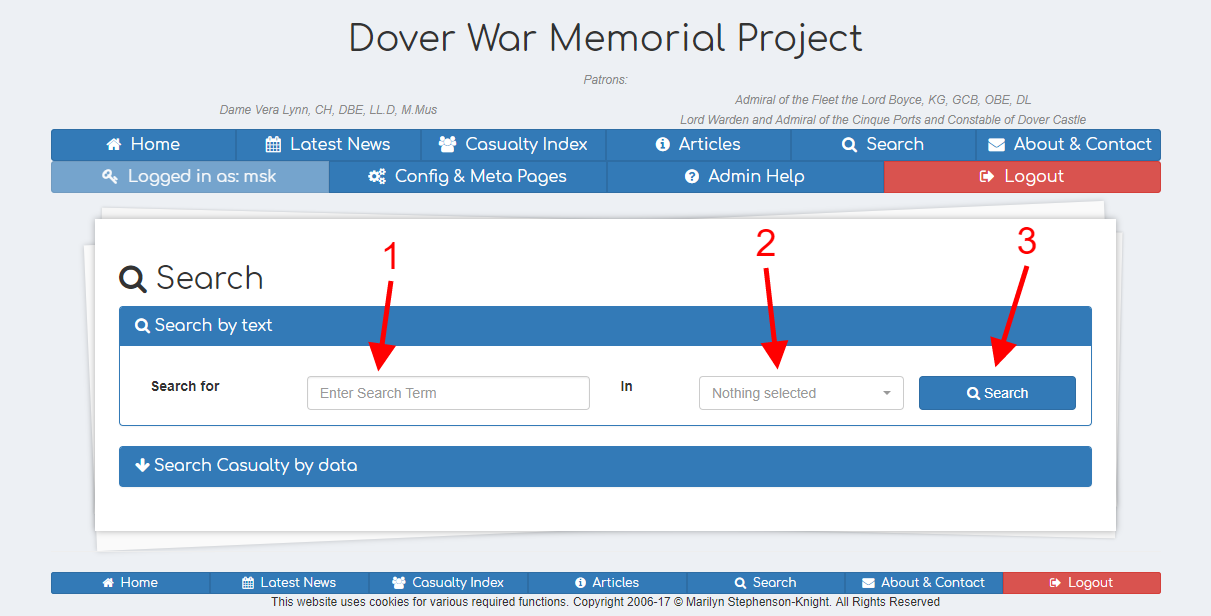
\includegraphics[width=.9\textwidth]{pics/text_search.png}
	\caption{Performing a Text Search}\label{fig:text_search}
\end{figure}

\marker{1}\ indicates the area to enter the search term, \marker{2}\ allows the user to select which areas of the site to search, and \marker{3}\ performs the search. The text based search is very powerful and can perform more than simple searches. Some main tips for use are displayed below \footnote{More examples are here: \url{https://dev.mysql.com/doc/refman/5.7/en/fulltext-boolean.html}, although the ranking is modified to boost casualties whose names contain any of the search terms}:

\begin{itemize}
\item Search terms are case insensitive.
\item Multiples words are treated as an ``or'' search - i.e. \texttt{dover war} will return all narratives containing \texttt{dover} or \texttt{war} or both.
\item Placing text within quote marks will search for those terms exactly.
\item Place a \texttt{+} in front of a word to ensure that word must be in results.
\item Place a \texttt{-} in front of a word to ensure that word must not be in results.
\item Place a \texttt{>} in front of a word to increase the relevance of that word.
\item Place a \texttt{<} in front of a word to decrease the relevance of that word.
\item Place a \texttt{*} to perform a wildcard search.  For example \texttt{Brit*} would return results for  \texttt{Britain}, \texttt{British}, and so on.
\item Common words (called ``stop words'', for example \texttt{the}, \texttt{at}) are ignored from the search.
\end{itemize}

Details of results are displayed in Section~\myref{ssec:view_search}.

\newpage
\FloatBarrier
\subsection{How do I perform a Data Search?}\label{ssec:data_search}
The main new feature of the search page, is the data search. This allows a user to search for all casualties who have a particular piece of data, for example, all those born on the same date, or all those who served in the Royal Navy. To view the full list of data items, click on \marker{1}\ in Figure~\myref{fig:data_search}.

\begin{figure}[h]
  \centering
 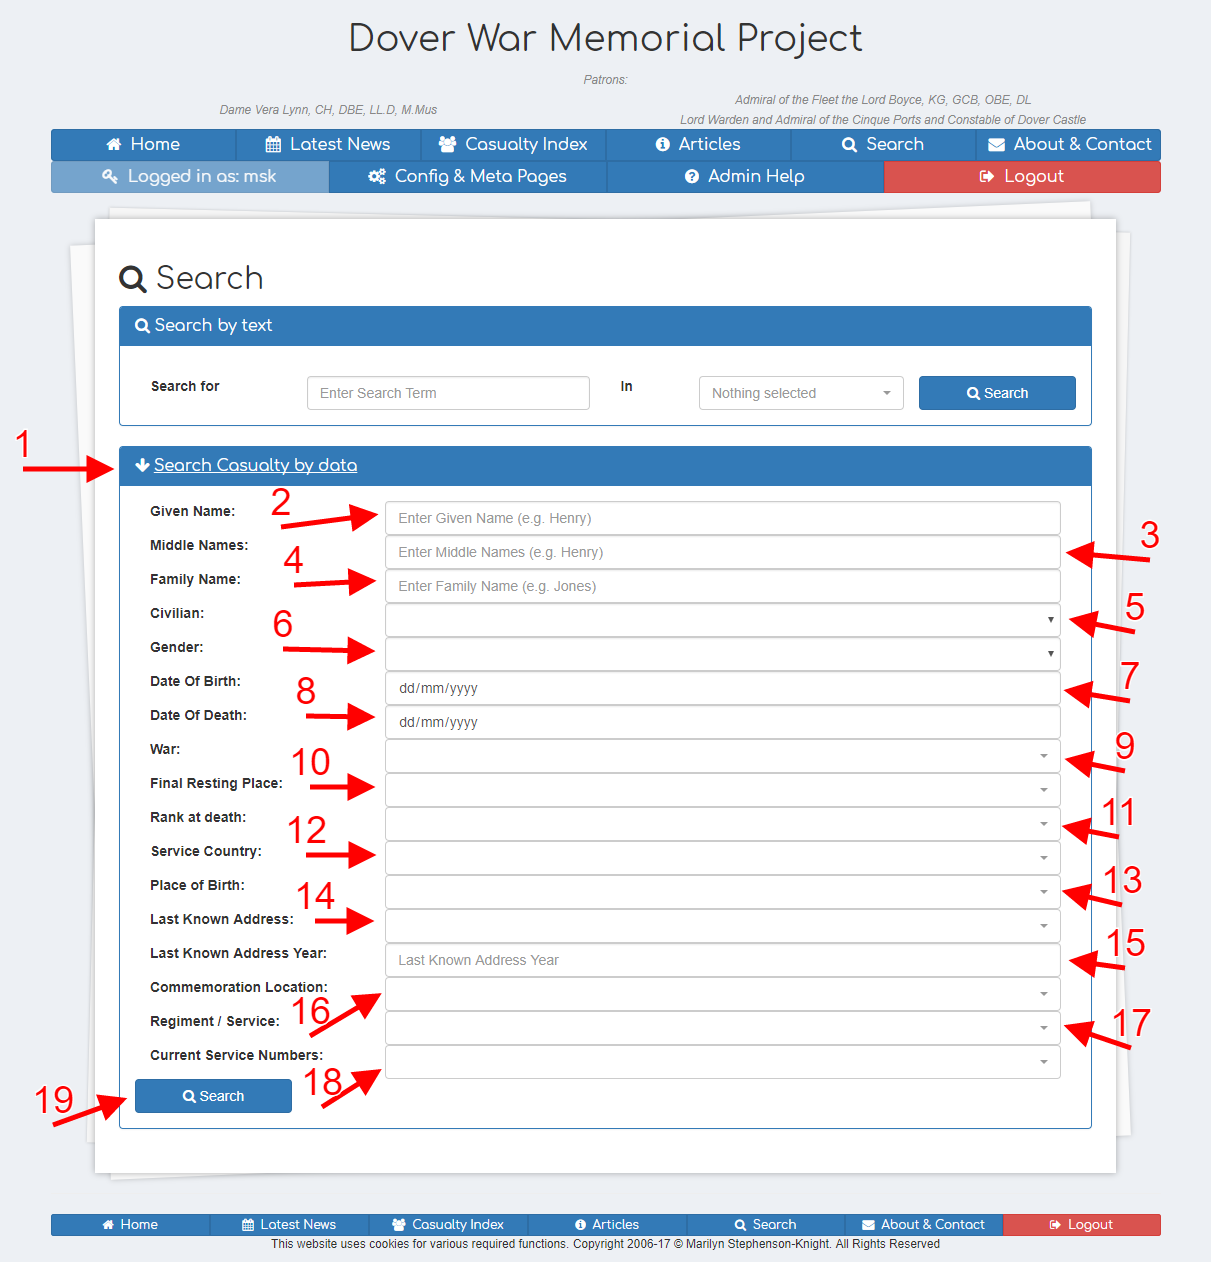
\includegraphics[width=.9\textwidth]{pics/data_search.png}
	\caption{Performing a Data Search}\label{fig:data_search}
\end{figure}

\marker{2}, \marker{3}, and \marker{4}\ allow the user to specify the name for the desired casualties. \marker{5}\ allows the specification of whether the casualties are civilians, while \marker{6}\ specifies their gender. \marker{7}\ and \marker{8}\ allow the user to specify the dates of birth and death respectively, while \marker{9}\ specifies the War. The final resting place for the casualties is shown by \marker{10}, with the rank at death being identified by \marker{11}. \marker{12}\ indicates the service country to be search, while \marker{13}\ shows the place of birth. The Last Known Address and the year of that address can be specified in \marker{14}\ and \marker{15}. \marker{16}\ allows the specification of any memorials the casualties may be commemorated on, with \marker{17}\ indicating the regiment / service and \marker{18}\ the service number. The search can be completed by clicking \marker{19}. Details of results are displayed in Section~\myref{ssec:view_search}.

\newpage
\FloatBarrier
\subsection{How do I view the Search Results?}\label{ssec:view_search}
Completing the either the text search (see Section~\myref{ssec:text_search}) or data search (see Section~\myref{ssec:data_search}) will display the results further down the page, as can be seen in Figure~\myref{fig:view_search}.

\begin{figure}[h]
  \centering
 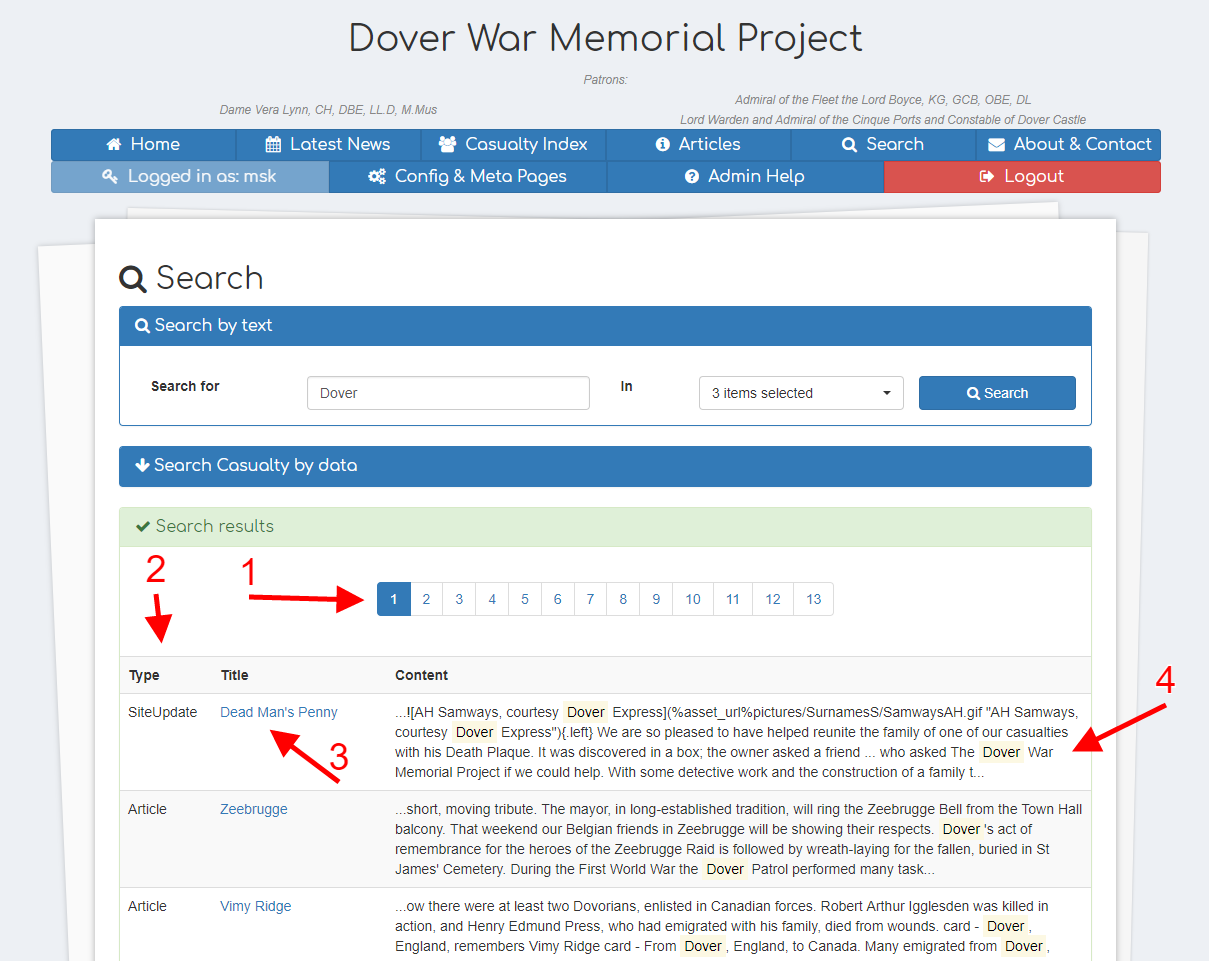
\includegraphics[width=.9\textwidth]{pics/view_search.png}
	\caption{Viewing Search Results}\label{fig:view_search}
\end{figure}

The list of numbers indicated by \marker{1}\ shows how many pages of results have been found, and which page is currently being viewed. \marker{2}\ indicates the type of result found, with \marker{3}\ showing the title of that result. Clicking this will navigate to the relevant article, memorial, casualty or site update. \marker{4}\ shows a preview of the results, with the search term highlighted.

If no search results can be found, the list of results will be displayed in a similar manner to Figure~\myref{fig:no_search}.

\begin{figure}[h]
  \centering
 
\includegraphics[width=.9\textwidth]{pics/no_search.png}
	\caption{Viewing No Search Results}\label{fig:no_search}
\end{figure}

\newpage
\FloatBarrier
\section{Configuration \& Meta Pages}\label{sec:config}
The configuration and meta pages section of the site is where the background changes are made to the site. Many of the items shown in this section are only viewable when logged in.

Meta pages are the ``other'' pages of the site. These come in two varieties:
\begin{enumerate}
\item Standalone pages (e.g. Contact), or
\item Sections of Text (e.g. at the top of the Articles list or the Home page)
\end{enumerate}

The idea of these is that is allows you to create (or edit) pages that do not fit into any other section and link to these as needed (for example, a contact page isn't really an article). It also allows the editing of narrative sections on pages that would otherwise be bland lists. There are a few meta pages that are required - for example the top of the Home page, or the Contact Us page, etc. These have all been added into the site already.

\begin{infoBox}
It is not possible to delete a meta page. There is a good reason for this. If a page was created that is no longer needed, simply remove any links to that page. If a page was accidentally deleted that was integral to the site (the Home page, for instance), that would be a disaster.
\end{infoBox}

\newpage
\FloatBarrier
\subsection{How do I view the config page?}\label{ssec:config}
The config page can be viewed by clicking on the \textit{Config \& Meta Page} button on the top menu bar when logged in. It should display similar to Figure~\myref{fig:view_meta}.

\begin{figure}[h]
  \centering
 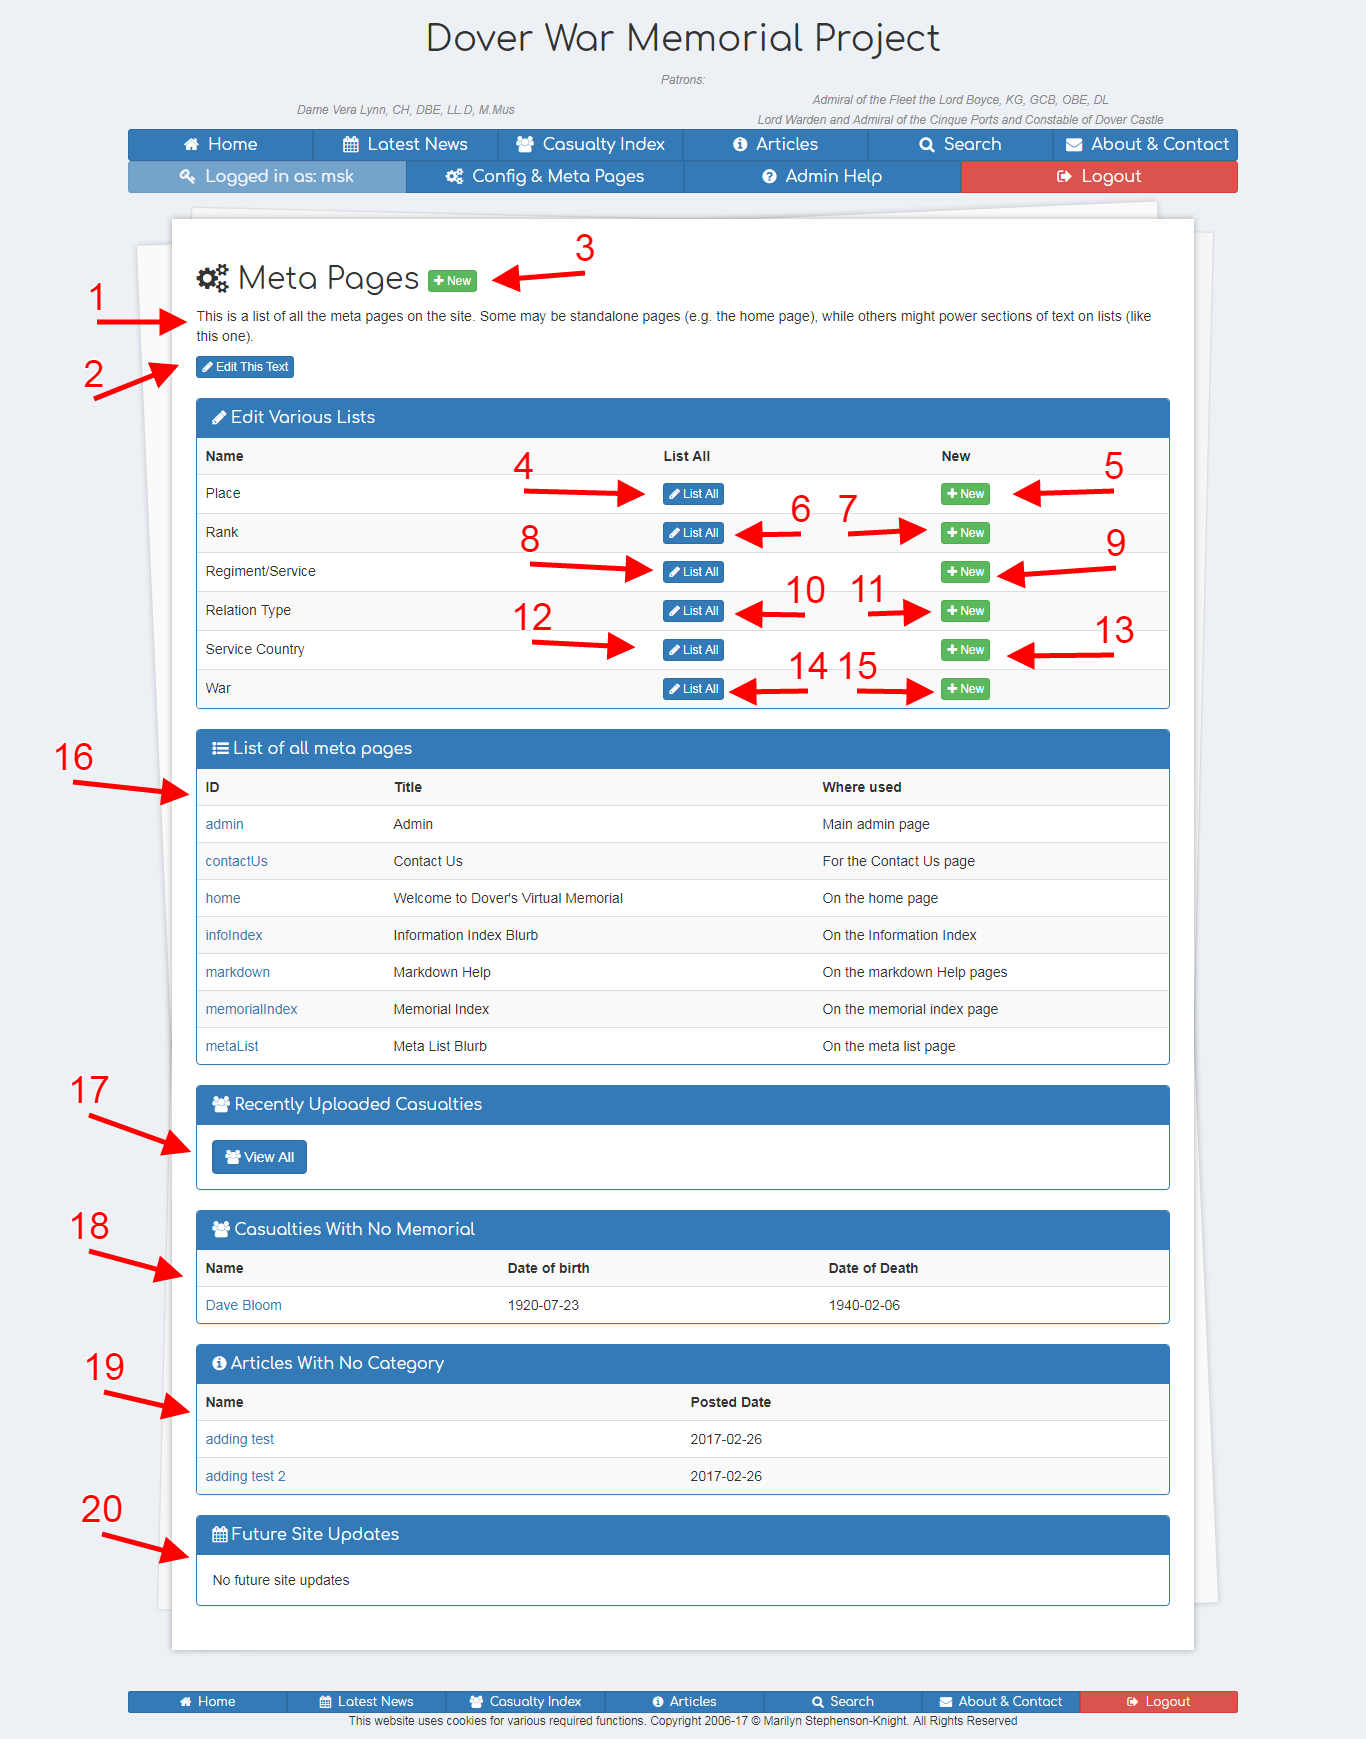
\includegraphics[width=.9\textwidth]{pics/view_meta.png}
	\caption{Config page}\label{fig:view_meta}
\end{figure}

\marker{1}\ is a small section of narrative that describes this page and is editable using \marker{2}, while \marker{3}\ allows the user to create a new meta page.

\marker{4}\ to \marker{15}\ allows the user to view a list of, or add to the list of Places, Ranks, Regiments, Relation Types, Countries and Wars (see Sections~\myref{ssec:view_place} --- \myref{ssec:edit_war}).

\marker{16}\ shows a list of the current meta pages and where they are used. The list of recently uploaded casualties can be displayed using \marker{17}\ (see Section~\ref{ssec:view_uploaded}). A list of casualties with no memorial is displayed as \marker{18}\ - this should normally be empty. A list of articles with no category is indicated by \marker{19}\ and this can be used to identify those articles who are linked to elsewhere. A list of site updates that are to be displayed at a future date are shown in a list indicated by \marker{20}.

\newpage
\FloatBarrier
\subsection{How do I edit a meta page?}
To edit a meta page, either find the page on the list of meta pages (\marker{16}\ in Figure~\myref{fig:view_meta}) and click the \textit{Edit} button next to the title, or click the \textit{Edit this text} button that appears on the page you wish you edit. Once the edit button has been clicked, a page should load similar to Figure~\myref{fig:edit_meta}.

\begin{figure}[h]
  \centering
 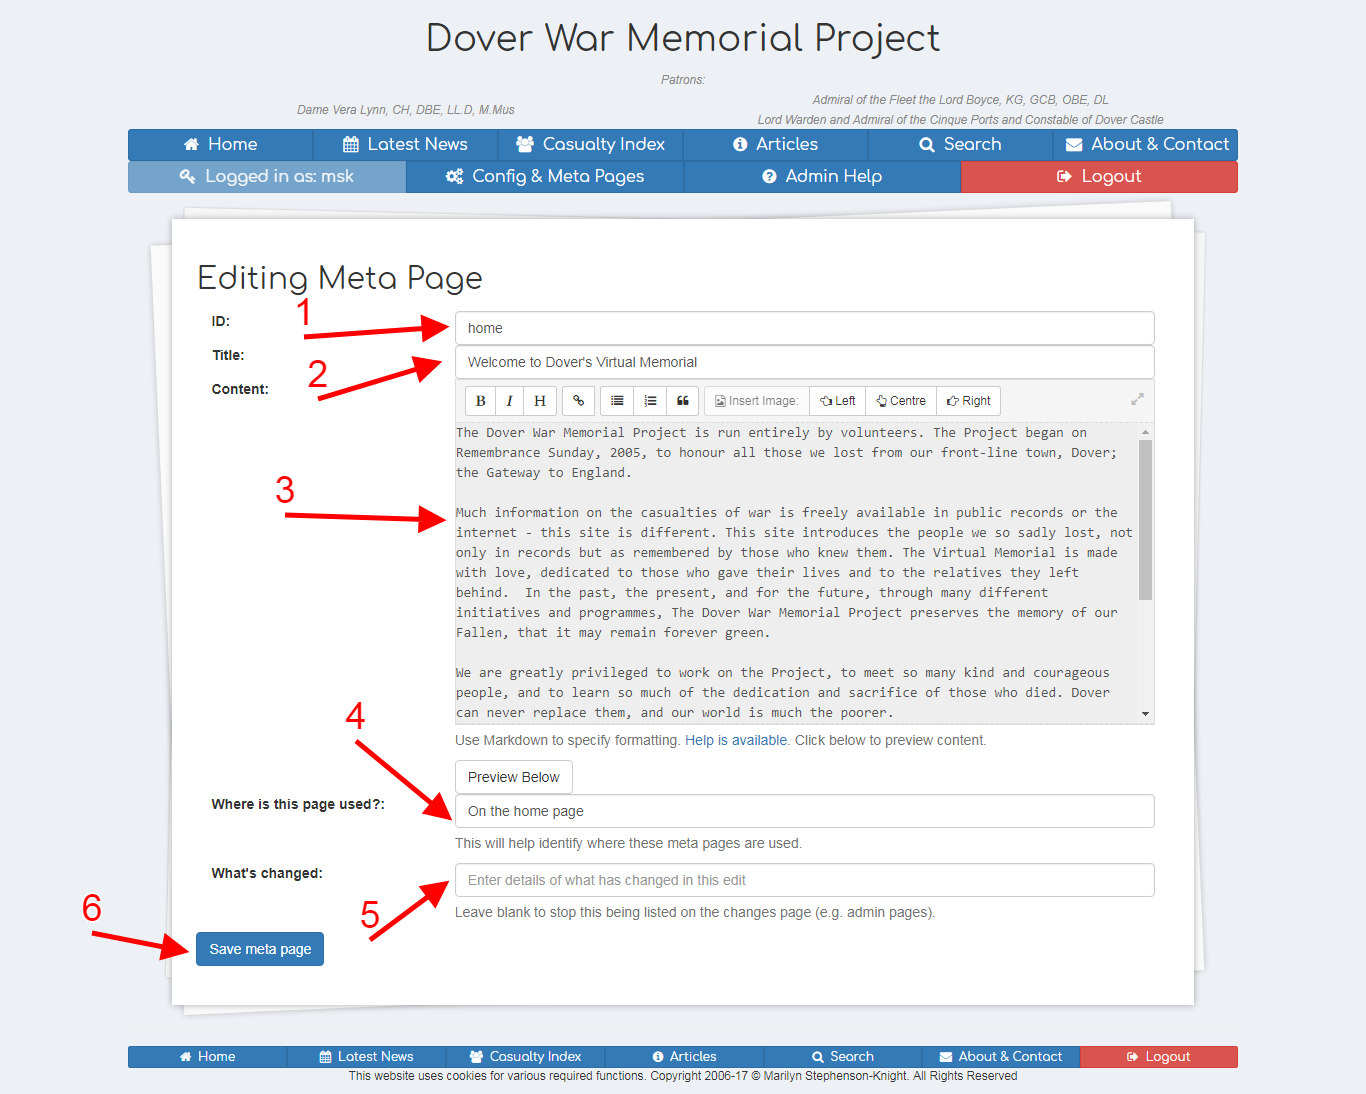
\includegraphics[width=.9\textwidth]{pics/edit_meta.png}
	\caption{Editing a meta page}\label{fig:edit_meta}
\end{figure}

\marker{1}\ indicates the ID of a meta page. This is used in the web address and is a unique identifier for the page. If the page is of the standalone variety, then the title indicated in \marker{2}\ will be displayed at the top of the page. The narrative section for the meta page is indicated by \marker{3}. An explanation of the buttons around this area is described in Section~\myref{ssec:narrative}. \marker{4}\ indicates where this meta page is used - this is displayed on the list of meta pages and helps to identify those with possibly obscure titles or IDs. As usual, \marker{5}\ indicates a box to add this change into the change log. \marker{6}\ allows the user to save this meta page.

\begin{warningBox}
The ID for a meta page MUST be unique.
\end{warningBox}

\newpage
\FloatBarrier
\subsection{How do I view a list of Places?} \label{ssec:view_place}
A list of Places can be viewed by clicking on \marker{4}\ in Figure~\myref{fig:view_meta}. A page will load similar to Figure~\myref{fig:view_place}.

\begin{figure}[h]
  \centering
 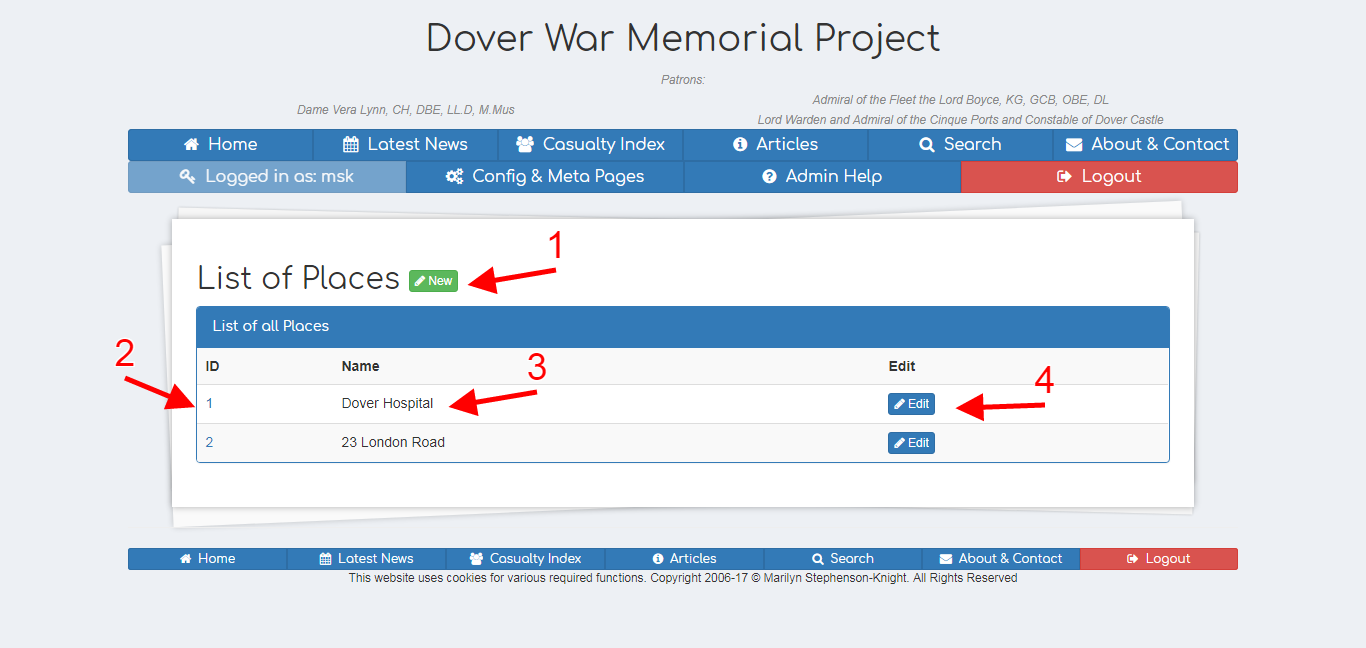
\includegraphics[width=.9\textwidth]{pics/view_place.png}
	\caption{Viewing a list of Places}\label{fig:view_place}
\end{figure}

\marker{1}\ allows the user to create a new Place. \marker{2}\ shows the ID of that place, with the name being shown in \marker{3}. \marker{4}\ allows the user to edit this Place.

\newpage
\FloatBarrier
\subsection{How do I Add, Edit or Delete a Place?}\label{ssec:edit_place}
A Place can be added by clicking on \marker{5}\ on Figure~\myref{fig:view_meta}, or by clicking on \marker{1}\ in Figure~\myref{fig:view_place}. A page will load similar to Figure~\myref{fig:edit_place}.

\begin{figure}[h]
  \centering
 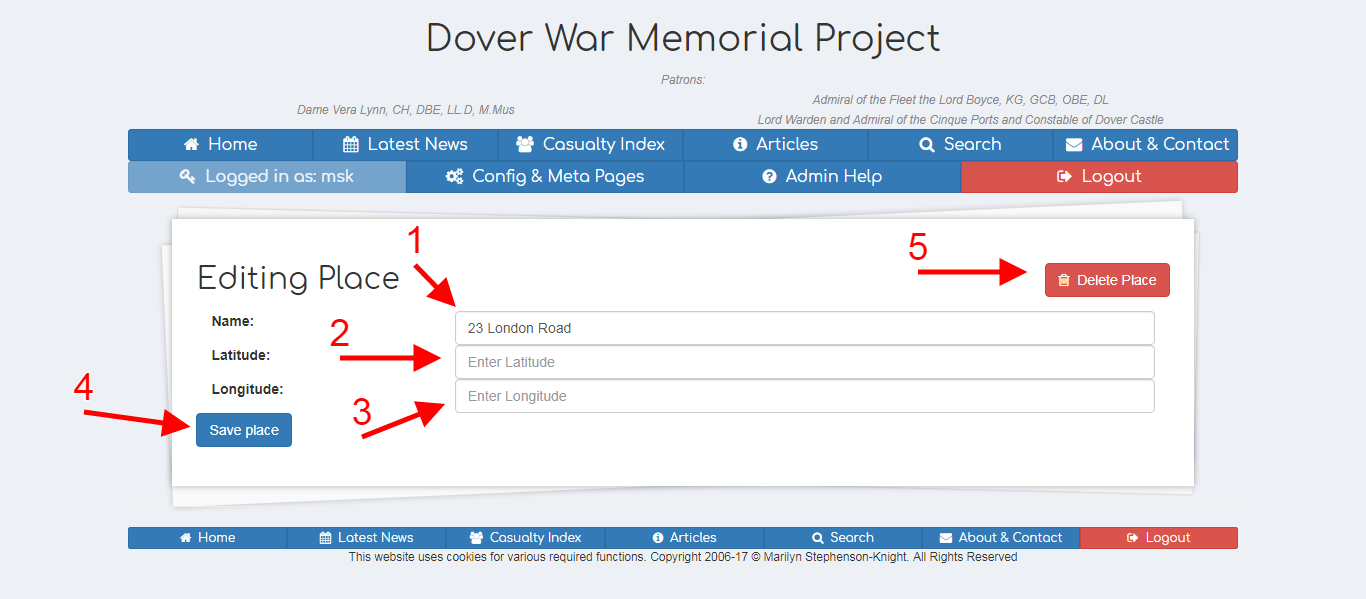
\includegraphics[width=.9\textwidth]{pics/edit_place.png}
	\caption{Editing a Place}\label{fig:edit_place}
\end{figure}

The name of the Place is indicated by \marker{1}, with the latitude and longitude being identified by \marker{2}\ and \marker{3}. The Place can be saved by \marker{4}\ and deleted by \marker{5}. Any casualty with this place will have it removed.

\begin{warningBox}
Deletion cannot be undone.
\end{warningBox} 

\newpage
\FloatBarrier
\subsection{How do I view a list of Ranks?}\label{ssec:view_rank}
A list of Ranks can be viewed by clicking on \marker{6}\ in Figure~\myref{fig:view_meta}. A page will load similar to Figure~\myref{fig:view_rank}.

\begin{figure}[h]
  \centering
 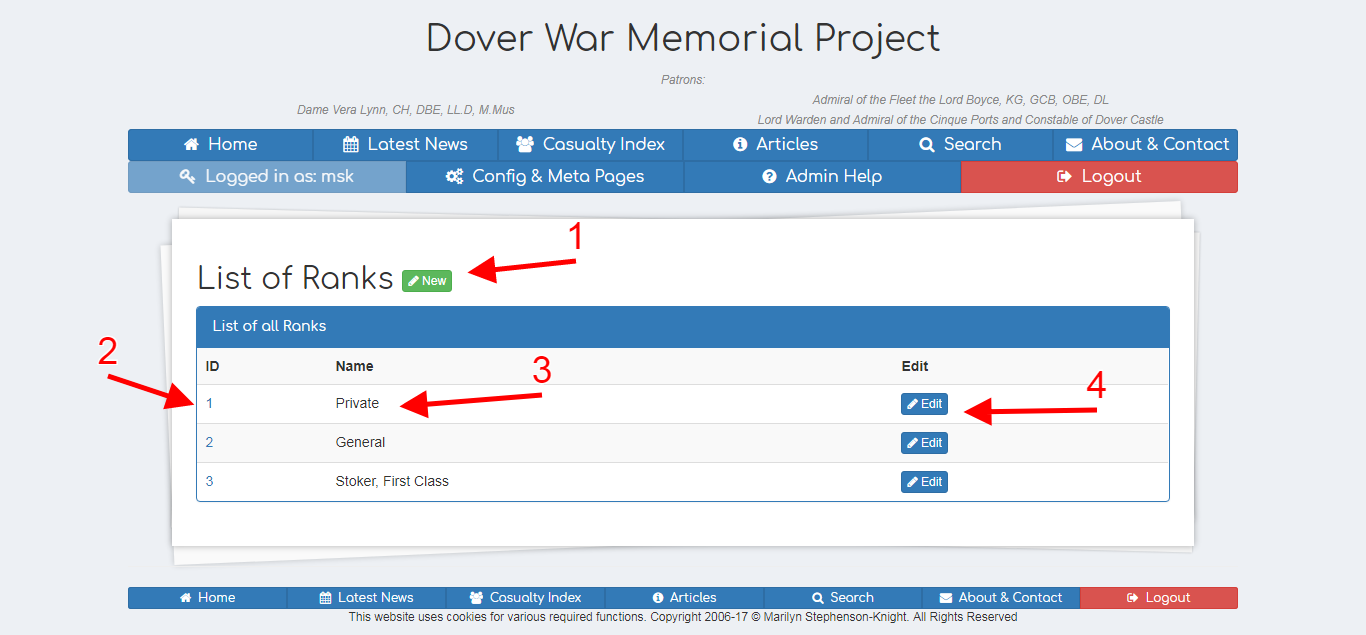
\includegraphics[width=.9\textwidth]{pics/view_rank.png}
	\caption{Viewing a list of Ranks}\label{fig:view_rank}
\end{figure}

\marker{1}\ allows the user to create a new Rank. \marker{2}\ shows the ID of that rank, with the name being shown in \marker{3}. \marker{4}\ allows the user to edit this Rank.

\newpage
\FloatBarrier
\subsection{How do I Add, Edit or Delete a Rank?}\label{ssec:edit_rank}
A Rank can be added by clicking on \marker{7}\ on Figure~\myref{fig:view_meta}, or by clicking on \marker{1}\ in Figure~\myref{fig:view_rank}. A page will load similar to Figure~\myref{fig:edit_rank}.

\begin{figure}[h]
  \centering
 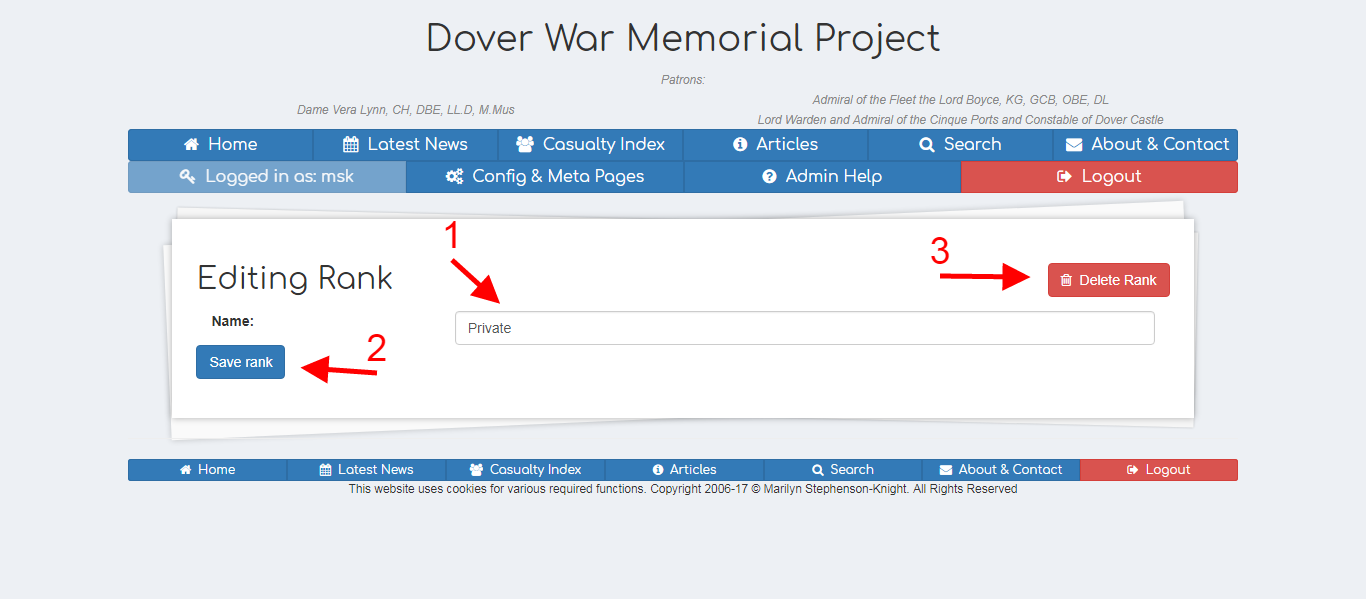
\includegraphics[width=.9\textwidth]{pics/edit_rank.png}
	\caption{Editing a Rank}\label{fig:edit_rank}
\end{figure}

The name of the Rank is indicated by \marker{1}. The Rank can be saved by \marker{2}\ and deleted by \marker{3}. Any casualty with this rank will have it removed.

\begin{warningBox}
Deletion cannot be undone.
\end{warningBox} 

\newpage
\FloatBarrier
\subsection{How do I view a list of Regiment / Service?} \label{ssec:view_regiment}
A list of Regiments / Services can be viewed by clicking on \marker{8}\ in Figure~\myref{fig:view_meta}. A page will load similar to Figure~\myref{fig:view_regiment}.

\begin{figure}[h]
  \centering
 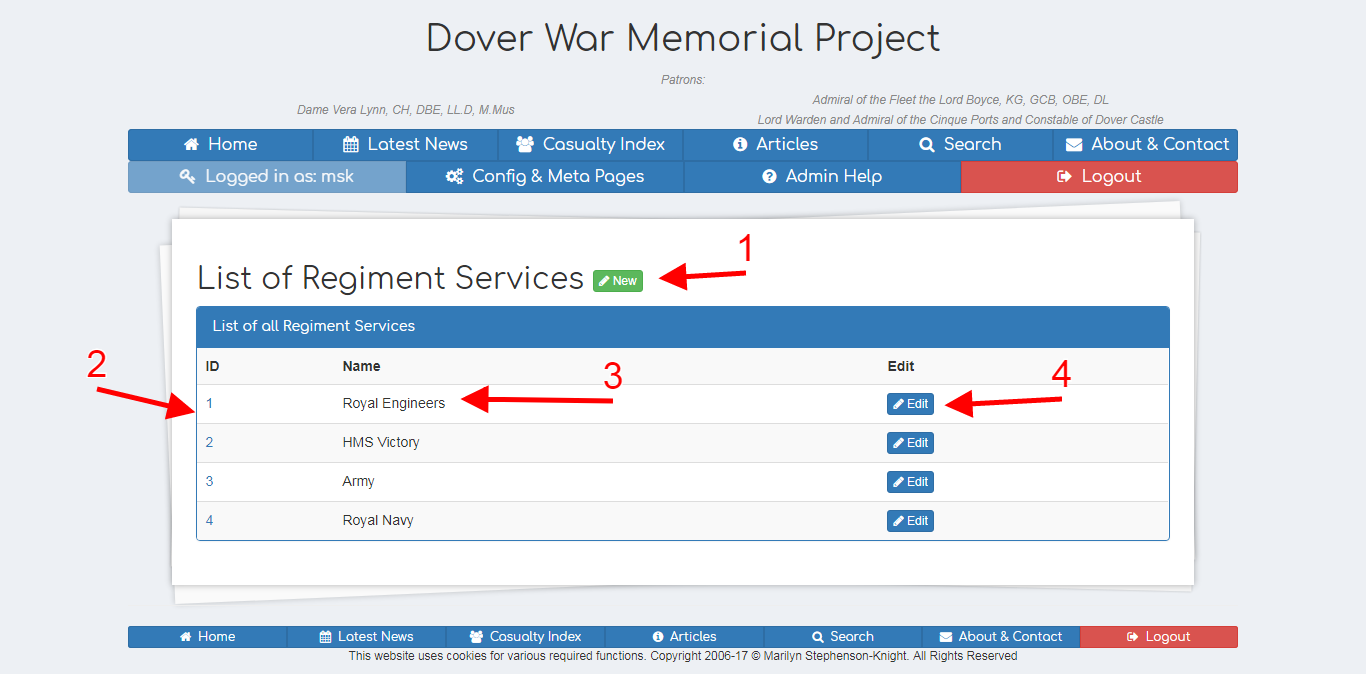
\includegraphics[width=.9\textwidth]{pics/view_regiment.png}
	\caption{Viewing a list of Regiments / Services}\label{fig:view_regiment}
\end{figure}

\marker{1}\ allows the user to create a new Regiment / Service. \marker{2}\ shows the ID of that regiment, with the name being shown in \marker{3}. \marker{4}\ allows the user to edit this Regiment / Service.

\newpage
\FloatBarrier
\subsection{How do I Add, Edit or Delete a Regiment / Service?} \label{ssec:edit_regiment}
A Regiment / Service can be added by clicking on \marker{9}\ on Figure~\myref{fig:view_meta}, or by clicking on \marker{1}\ in Figure~\myref{fig:view_regiment}. A page will load similar to Figure~\myref{fig:edit_regiment}.

\begin{figure}[h]
  \centering
 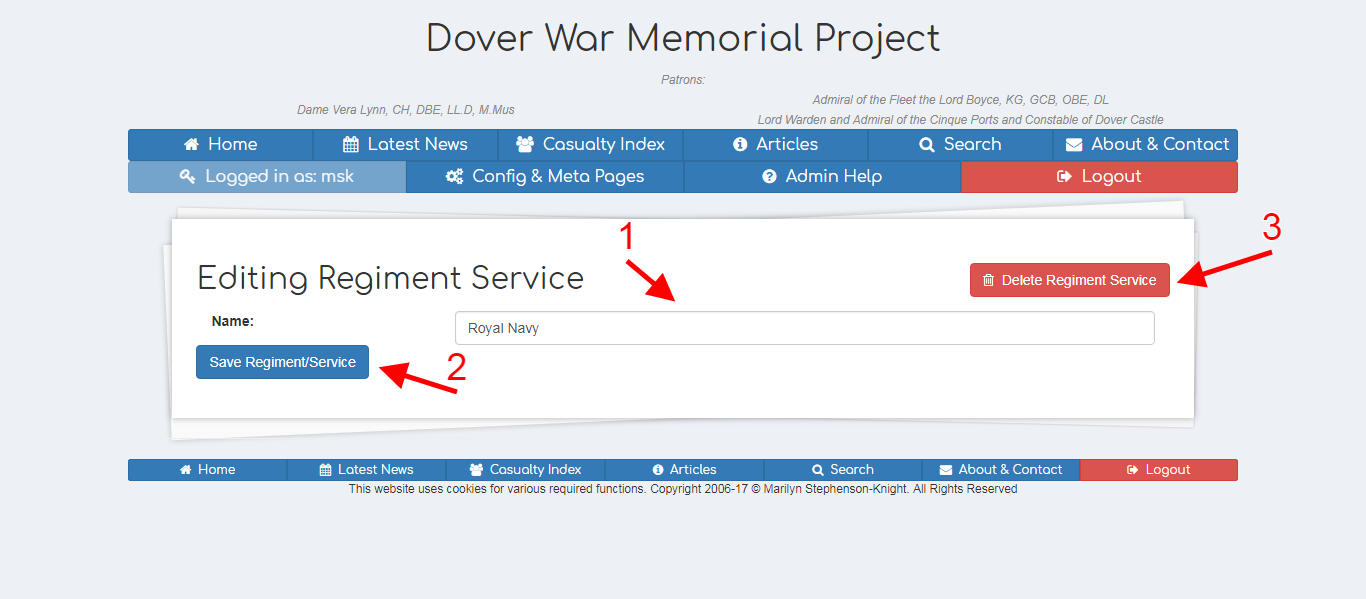
\includegraphics[width=.9\textwidth]{pics/edit_regiment.png}
	\caption{Editing a Regiment / Service}\label{fig:edit_regiment}
\end{figure}

The name of the Regiment / Service is indicated by \marker{1}. The Regiment / Service can be saved by \marker{2}\ and deleted by \marker{3}. Any casualty with this Regiment / Service will have it removed.

\begin{warningBox}
Deletion cannot be undone.
\end{warningBox} 


\newpage
\FloatBarrier
\subsection{How do I view a list of Relation Types?} \label{ssec:view_relation}

A list of Relation Types can be viewed by clicking on \marker{10}\ in Figure~\myref{fig:view_meta}. A page will load similar to Figure~\myref{fig:view_relation}.

\begin{figure}[h]
  \centering
 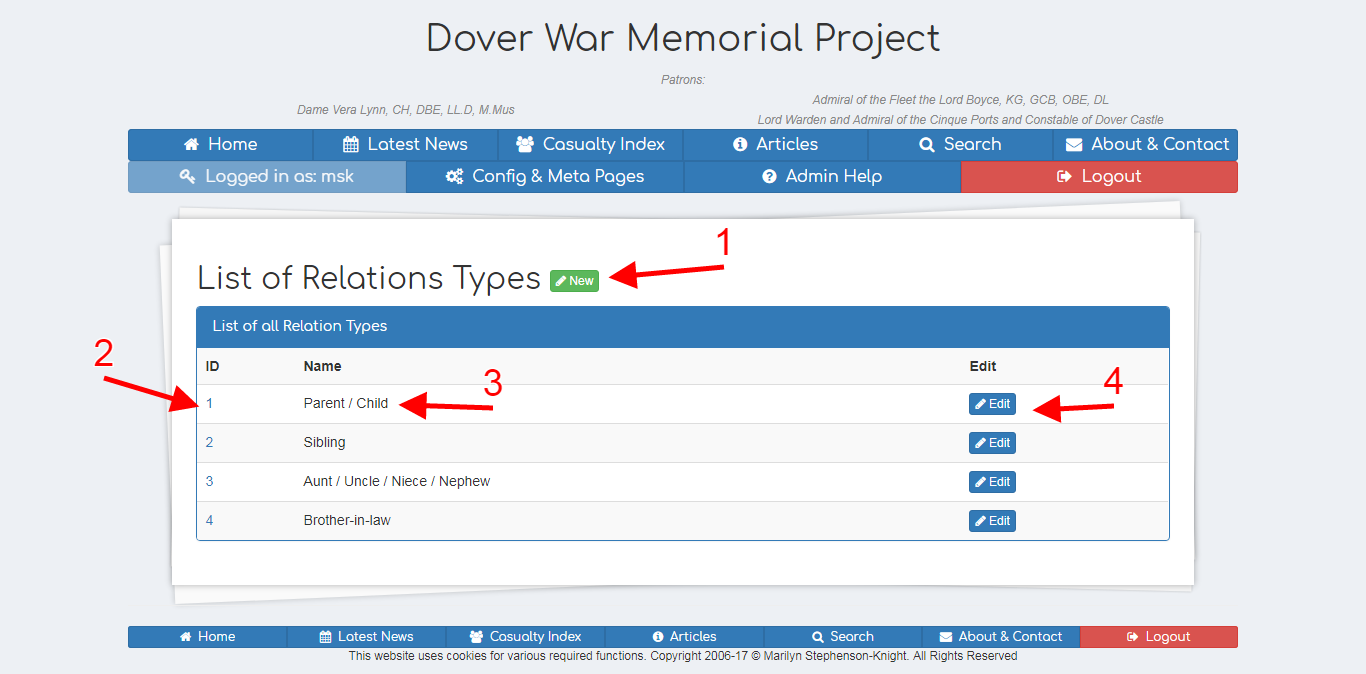
\includegraphics[width=.9\textwidth]{pics/view_relation.png}
	\caption{Viewing a list of Relation Types}\label{fig:view_relation}
\end{figure}

\marker{1}\ allows the user to create a new Relation Type. \marker{2}\ shows the ID of that Relation Type, with the name being shown in \marker{3}. \marker{4}\ allows the user to edit this Relation Type.

\begin{infoBox}
A relation has no direction, so these types have long names to cover this.
\end{infoBox}

\newpage
\FloatBarrier
\subsection{How do I Add, Edit or Delete a Relation Type?} \label{ssec:edit_relation}

A Relation Type can be added by clicking on \marker{11}\ on Figure~\myref{fig:view_meta}, or by clicking on \marker{1}\ in Figure~\myref{fig:view_relation}. A page will load similar to Figure~\myref{fig:edit_relation}.

\begin{figure}[h]
  \centering
 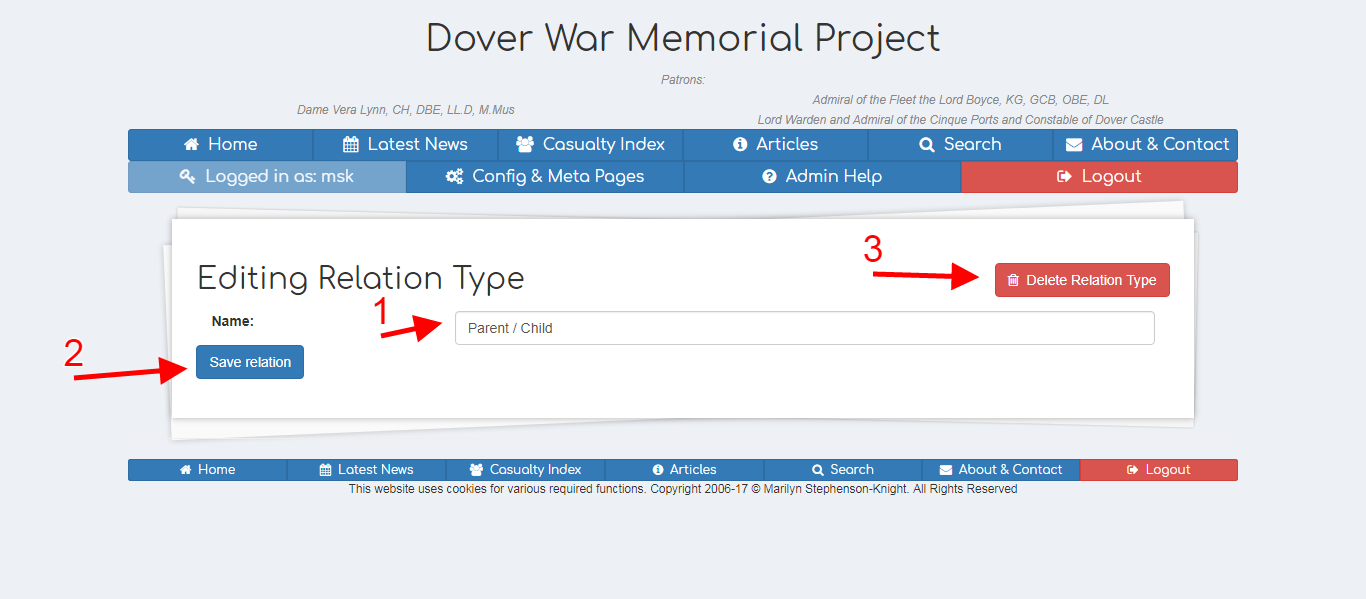
\includegraphics[width=.9\textwidth]{pics/edit_relation.png}
	\caption{Editing a Relation Type}\label{fig:edit_relation}
\end{figure}

The name of the Relation Type is indicated by \marker{1}. The Relation Type can be saved by \marker{2}\ and deleted by \marker{3}. Any casualties with this Relation Type will have that relation removed.

\begin{warningBox}
Deletion cannot be undone.
\end{warningBox} 

\newpage
\FloatBarrier
\subsection{How do I view a list of Service Countries?} \label{ssec:view_country}

A list of Service Countries can be viewed by clicking on \marker{12}\ in Figure~\myref{fig:view_meta}. A page will load similar to Figure~\myref{fig:view_country}.

\begin{figure}[h]
  \centering
 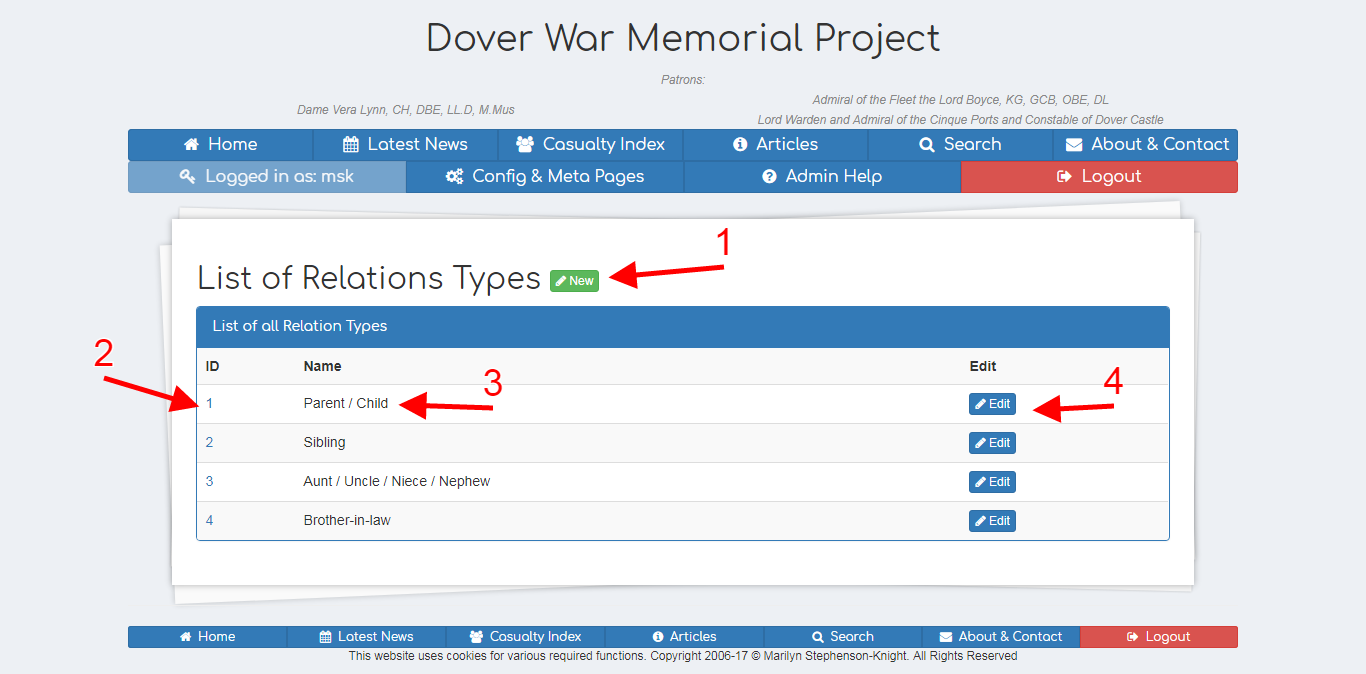
\includegraphics[width=.9\textwidth]{pics/view_relation.png}
	\caption{Viewing a list of Service Countries}\label{fig:view_country}
\end{figure}

\marker{1}\ allows the user to create a new Service Country. \marker{2}\ shows the ID of that Service Country, with the name being shown in \marker{3}. \marker{4}\ allows the user to edit this Service Country.

\newpage
\FloatBarrier
\subsection{How do I Add, Edit or Delete a Service Country?} \label{ssec:edit_country}

A Service Country can be added by clicking on \marker{13}\ on Figure~\myref{fig:view_meta}, or by clicking on \marker{1}\ in Figure~\myref{fig:view_country}. A page will load similar to Figure~\myref{fig:edit_country}.

\begin{figure}[h]
  \centering
 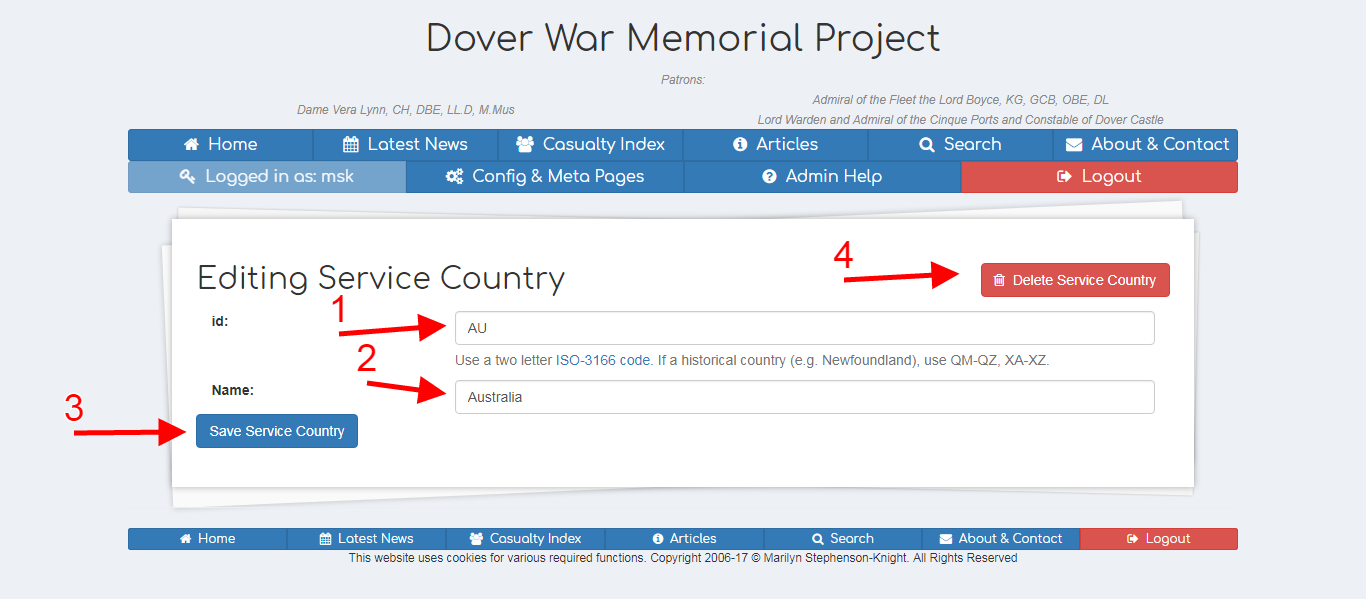
\includegraphics[width=.9\textwidth]{pics/edit_country.png}
	\caption{Editing a Service Country}\label{fig:edit_country}
\end{figure}

The ID of the Service Country is specified by \marker{1} (according to ISO 3166\footnote{\url{https://en.wikipedia.org/wiki/ISO_3166-1_alpha-2}}), with the name being shown by \marker{2}. The Service Country can be saved by \marker{3}\ and deleted by \marker{4}. Any casualties with this Service Country will have that data removed.

\begin{warningBox}
Deletion cannot be undone.
\end{warningBox} 

\begin{infoBox}
A country's ID must be their two letter ISO-3166 code. If editing a historical country (e.g. Newfoundland), use any letters in the range of QM---QZ, XA---XZ. All countries needed should be already added.
\end{infoBox}

\newpage
\FloatBarrier
\subsection{How do I view a list of Wars?} \label{ssec:view_war}
A list of Wars can be viewed by clicking on \marker{14}\ in Figure~\myref{fig:view_meta}. A page will load similar to Figure~\myref{fig:view_war}.

\begin{figure}[h]
  \centering
 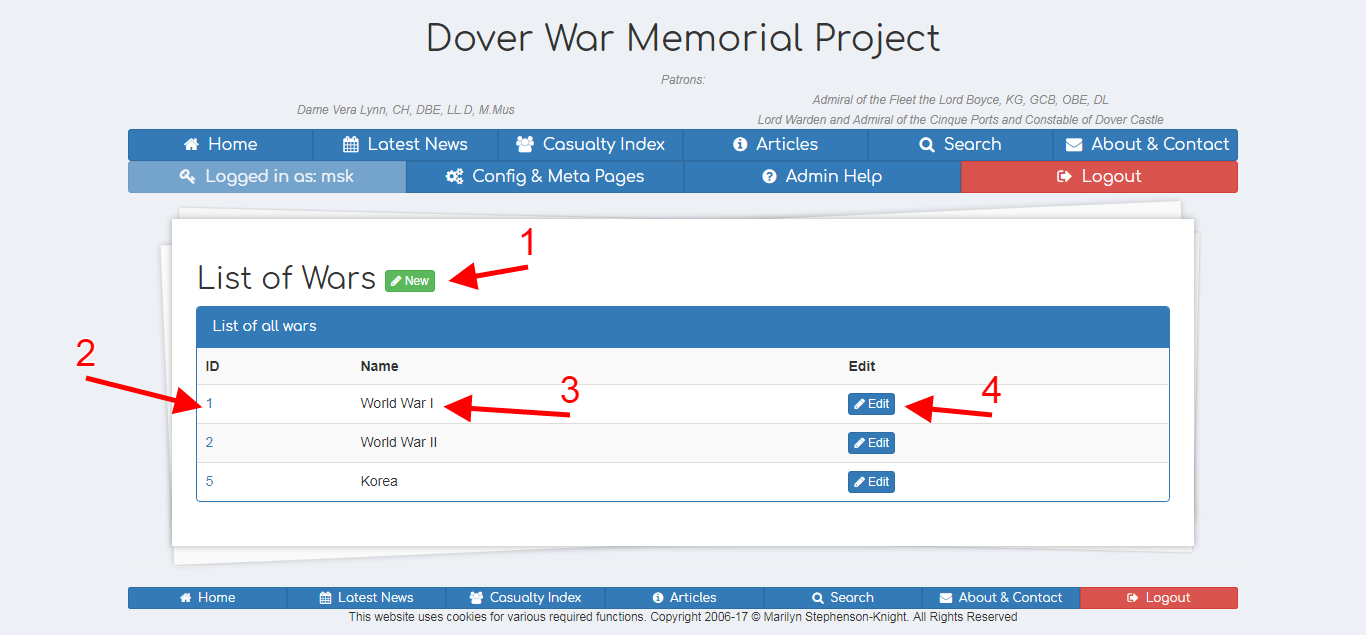
\includegraphics[width=.9\textwidth]{pics/view_war.png}
	\caption{Viewing a list of Wars}\label{fig:view_war}
\end{figure}

\marker{1}\ allows the user to create a new War. \marker{2}\ shows the ID of that War, with the name being shown in \marker{3}. \marker{4}\ allows the user to edit this War.

\newpage
\FloatBarrier
\subsection{How do I Add, Edit or Delete a War?} \label{ssec:edit_war}
A War can be added by clicking on \marker{15}\ on Figure~\myref{fig:view_meta}, or by clicking on \marker{1}\ in Figure~\myref{fig:view_war}. A page will load similar to Figure~\myref{fig:edit_war}.

\begin{figure}[h]
  \centering
 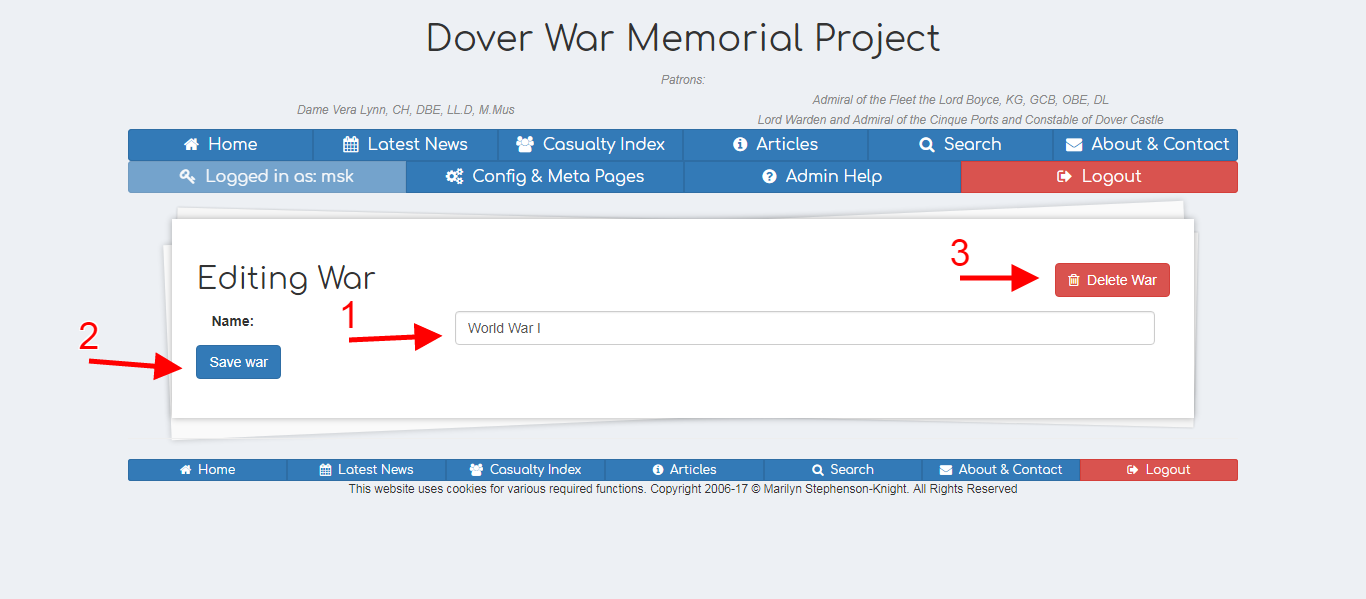
\includegraphics[width=.9\textwidth]{pics/edit_war.png}
	\caption{Editing a War}\label{fig:edit_war}
\end{figure}

The name of the War is indicated by \marker{1}. The War can be saved by \marker{2}\ and deleted by \marker{3}. Any casualties with this War will have that data removed.

\begin{warningBox}
Deletion cannot be undone.
\end{warningBox} 

\newpage
\FloatBarrier
\subsection{How do I view a List of Recently Imported Casualties?}\label{ssec:view_uploaded}
A list of recently imported casualties is available by clicking the button indicated by \marker{17}\ in Figure~\myref{fig:view_meta}. Over time, this list should eventually be empty. A page will load similar to the fragment shown in Figure~\myref{fig:view_uploaded}.

\begin{figure}[h]
  \centering
 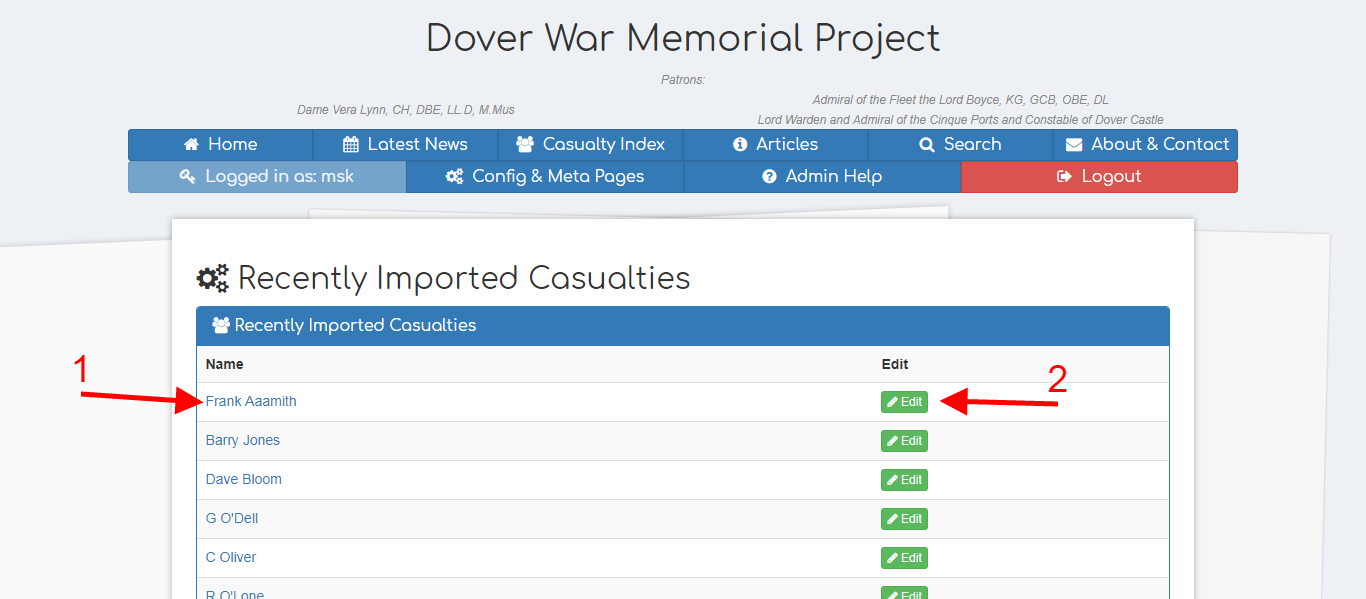
\includegraphics[width=.9\textwidth]{pics/view_uploaded.png}
	\caption{Viewing the list of Recently Imported Casualties}\label{fig:view_uploaded}
\end{figure}

The name of the casualty is shown by \marker{1}, with a link to their edit page shown by \marker{2}.

\newpage
\FloatBarrier
\section{Others}
This section contains tasks and other features which do not fit nicely into the other categories.

\subsection{How does the site look on mobile?}\label{ssec:mobile}
The new site is responsive and will adjust its layout based on the screen size. As the size of the screen reduces, several changes occur:
\begin{itemize}
\item The labels on the menu bars disappear, leaving only the icons
\item The labels on the menu bars disappear, leaving only the icons. The ``paper'' effect on the main display area is also replaced with a lozenge shape with a shadow. This reduces the wasted space on the left and right of the screen.
\item The ``patrons'' section also disappears. This saves a huge amount of space at the top of the screen and stops the user having to scroll down to the main content.
\item The panels on the home page that are side-by-side appear below one another. They would appear too crushed side-by-side on most mobile devices.
\item The map on memorial pages appear below the narrative rather than next to them. This again stops horizontal scrolling or making items too squashed.
\end{itemize}
An example of the home page on mobile is shown as Figure~\myref{fig:mobile}.

\begin{figure}[h]
  \centering
 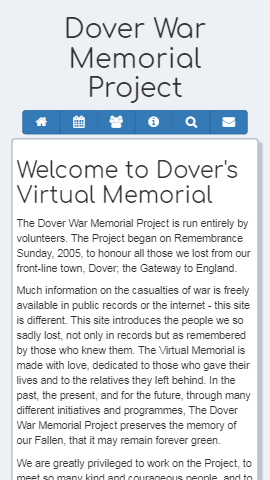
\includegraphics[height=.45\textheight]{pics/mobile.png}
	\caption{Viewing the home page on a mobile phone}\label{fig:mobile}
\end{figure}

\newpage
\FloatBarrier
\subsection{How do I use the Narrative Buttons?}\label{ssec:narrative}
The narrative buttons are used to create styling and to add pictures and links to the various narrative sections throughout the site. All narrative sections throughout the site operate in the same manner. Although there are buttons, the text is formatted using a language called \texttt{Markdown}. This has simpler syntax to HTML and also has the benefit of not breaking other areas of the site if invalid styling is entered. The buttons should handle most cases, but may not be great at ``undoing'' a style change. The narrative section is displayed in a similar manner to Figure~\myref{fig:markdown}.

\begin{figure}[h]
  \centering
 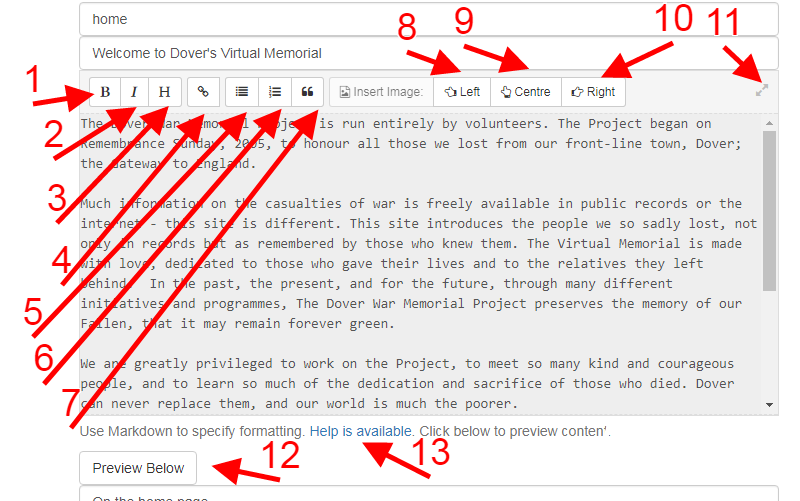
\includegraphics[width=.9\textwidth]{pics/markdown.png}
	\caption{Narrative Buttons}\label{fig:markdown}
\end{figure}

The buttons labelled \marker{1}\ to \marker{10}\ are described below in Table~\myref{tbl:markdown}.

The Left, Centre and Right image buttons will ask for an address to the picture and a caption before placing the image to the left, right or middle of the text. The address asked, must be relative to the assets folder, so that is a file is in \texttt{assets/pictures/me.png}, the user should enter \texttt{me.png}. The caption provided will be displayed if the image cannot be loaded, or a user has images disabled, or is using some text-to-speech software if they have a sight problem.

The link button will also ask for a address. It is fine to enter a full, absolute link in here, for example \texttt{www.doverwarmemorial.org.uk/casualty/view/3}.

The editing window can be made fullscreen by clicking the button indicated by \marker{11}\ and the markdown can be previewed by \marker{12}. This preview is shown below the editing window. This help is repeated in a similar manner in the link provided by \marker{13}.

\begin{landscape}
\begin{table}[h]
\centering
\begin{tabular}{llll}
 & \textbf{Name}  & \textbf{Markdown}                                                                                                                                                & \textbf{Display} \\ \hline
\marker{1}    & Bold           & \texttt{**Dover**}                                                                                                                                                        & \textbf{Dover}   \\
\marker{2}    & Italics        & \texttt{\_Dover\_}                                                                                                                                                        & \textit{Dover}   \\
\marker{3}    & Heading        & \texttt{\#\#\# Dover}                                                                                                                                                     &  
\includegraphics[scale=0.8]{pics/heading.png}       \\
\marker{4}    & Link           & \texttt{{[}Google{]}(http://google.com)}                                                                                                                                  &     
\includegraphics[scale=0.8]{pics/link.png}             \\
\marker{5}    & Bullet List    & \begin{tabular}[c]{@{}l@{}}\texttt{- item 1}\\\texttt{- item 2}\end{tabular}                                                                                                      &   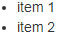
\includegraphics[scale=0.8]{pics/list.png}   \\
\marker{6}    & Numbered List  & \begin{tabular}[c]{@{}l@{}}\texttt{1. item 1}\\\texttt{2. item 2}\end{tabular}                                                                                                    &   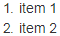
\includegraphics[scale=0.8]{pics/number.png}   \\
\marker{7}    & Quotation      & \texttt{\textgreater\ Dover}                                                                                                                                               &   
\includegraphics[scale=0.8]{pics/quote.png}  \\
\marker{8}    & Image (Left)   & \texttt{!{[}Picture of face{]}(\%asset\_url\%pictures/faces/me.png "Picture of face")\{.left\}} & See above \\
\marker{9}    & Image (Centre) & \texttt{!{[}Picture of face{]}(\%asset\_url\%pictures/faces/me.png "Picture of face")\{.middle\}}                                             &  See above \\
\marker{10}   & Image (Right)  & \texttt{!{[}Picture of face{]}(\%asset\_url\%pictures/faces/me.png "Picture of face")\{.right\}}                                              & See above \\
\marker{-}   & Paragraph      & An empty line between sections of text                                                                                                                           &                 
\end{tabular}
\caption{Styling guide}
\label{tbl:markdown}
\end{table}
\end{landscape}

\end{document}